\section{Basic Acquisition Functions}
%----------------------------------------------------------------------
%----------------------------------------------------------------------
\begin{frame}[c]{Acquisition Functions}
\framesubtitle{Description}
\comment{Refine, maybe consult a tutorial.}
\begin{itemize}
    \item \cemph{red}{Problem:} Given the surrogate function $\iter{\surro}(\conf)$ at the $\bocount\,$th iteration of BO, choose the "best" candidate $\iter{\conf}\in \pcs$ to evaluate $\cost(\conf)$ at next
\pause
\smallskip
    \item \cemph{violet}{Solution(?):} Evaluate at a global minimum of $\iter{\surro}(\conf)$ 
    \item \cemph{red}{Issues:}
    \begin{itemize}
        \item The surrogate function is inaccurate. The global optimum of $\iter{\surro}(\conf)$ does not necessarily yield the ``best'' $\cost(\conf)$. This is exactly why every candidate $\conf$ has an assosciated variance $\variance(\conf)$
        \item Considering our uncertainty, we also need to consider the \alert{exploration-exploitation trade-off}
    \end{itemize}
\pause
\smallskip
    \pause
    \item \cemph{blue}{Real Solution}: Use a heuristic estimate $\acq(\cdot)$ aka \alert{acquisition function} that trades of exploration and exploitation!
\end{itemize}

\end{frame}
%-----------------------------------------------------------------------
\begin{frame}[c]{Acquisition Functions}
\framesubtitle{Types}
\begin{itemize}
    \item Basic Acquisition Functions
    \begin{itemize}
        \item Probability of Improvement - PI
        \item Expected Improvement - EI
        \item Lower/Upper Confidence Bounds - LCB/UCB
        \item Thompson Sampling - TS
    \end{itemize}
    \item Advanced Acquisition Functions
    \begin{itemize}
        \item Knowledge Gradient
        \item Entropy Search
    \end{itemize}
\end{itemize}

\end{frame}
%-----------------------------------------------------------------------
%\subsection{Basic Acquisition Functions}
\begin{frame}[c]{Basic Acquisition Functions - PI}
\framesubtitle{Probability of Improvement - Concept}
\begin{figure}
  \centering
  \begin{tikzpicture}
    \node<+> (img1) {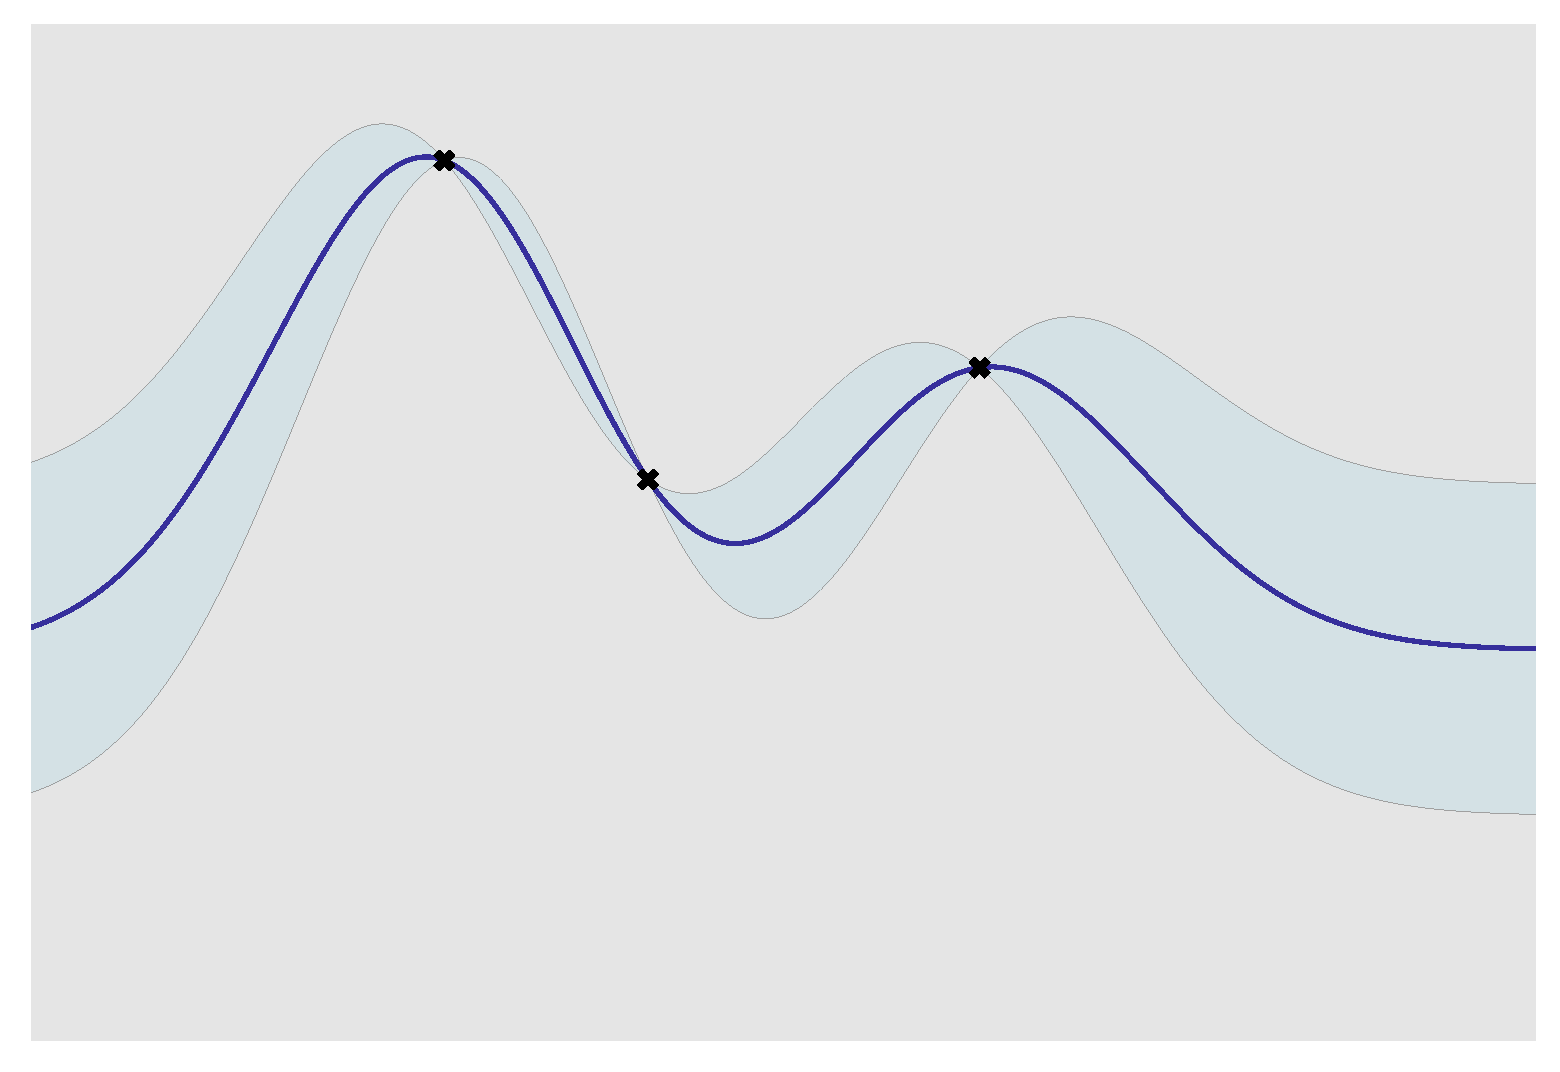
\includegraphics[width=.7\linewidth, height=0.7\textheight, keepaspectratio=true]{images/acq_func_images/pi_1.pdf}};
    \node<.> [below=0.01\belowcaptionskip of img1, align=center]{GP fit on 3 observations};

    \node<+> (img2) {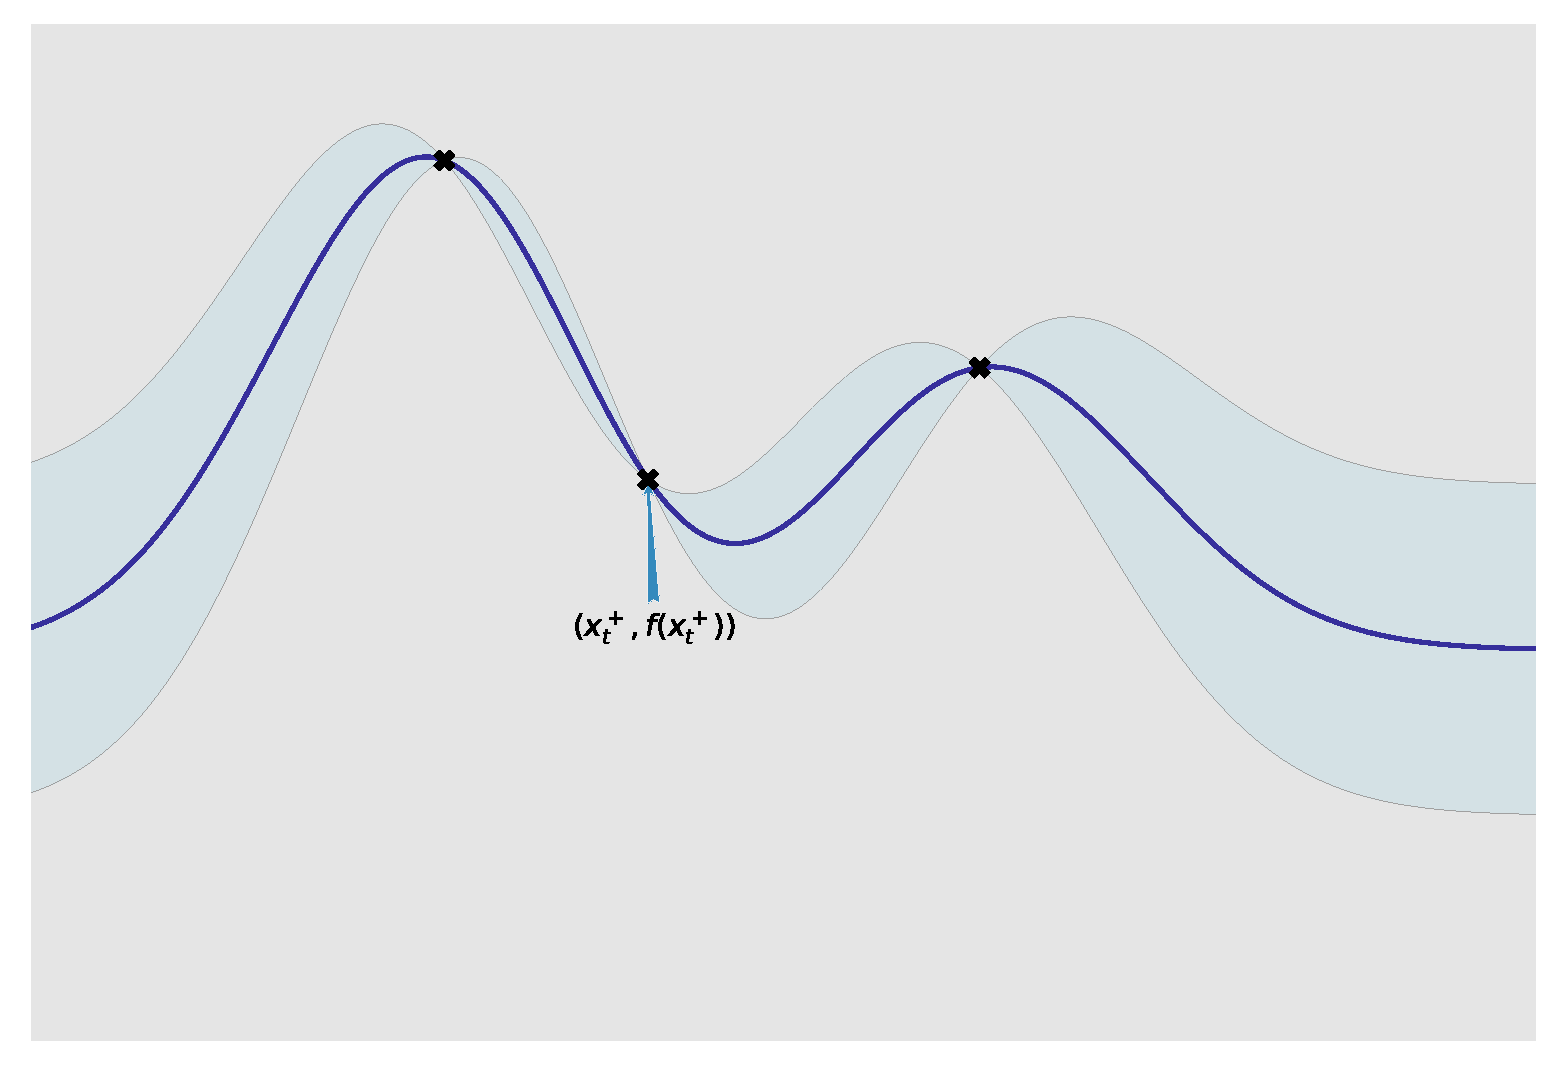
\includegraphics[width=.7\linewidth, height=0.7\textheight, keepaspectratio=true]{images/acq_func_images/pi_2.pdf}};
    \node<.> [below=0.01\belowcaptionskip of img2, align=center]{Current incumbent $\incumbent[\bocount-1]$ and it's observed value $\cost(\incumbent[\bocount-1])$};

    \node<+> (img3) {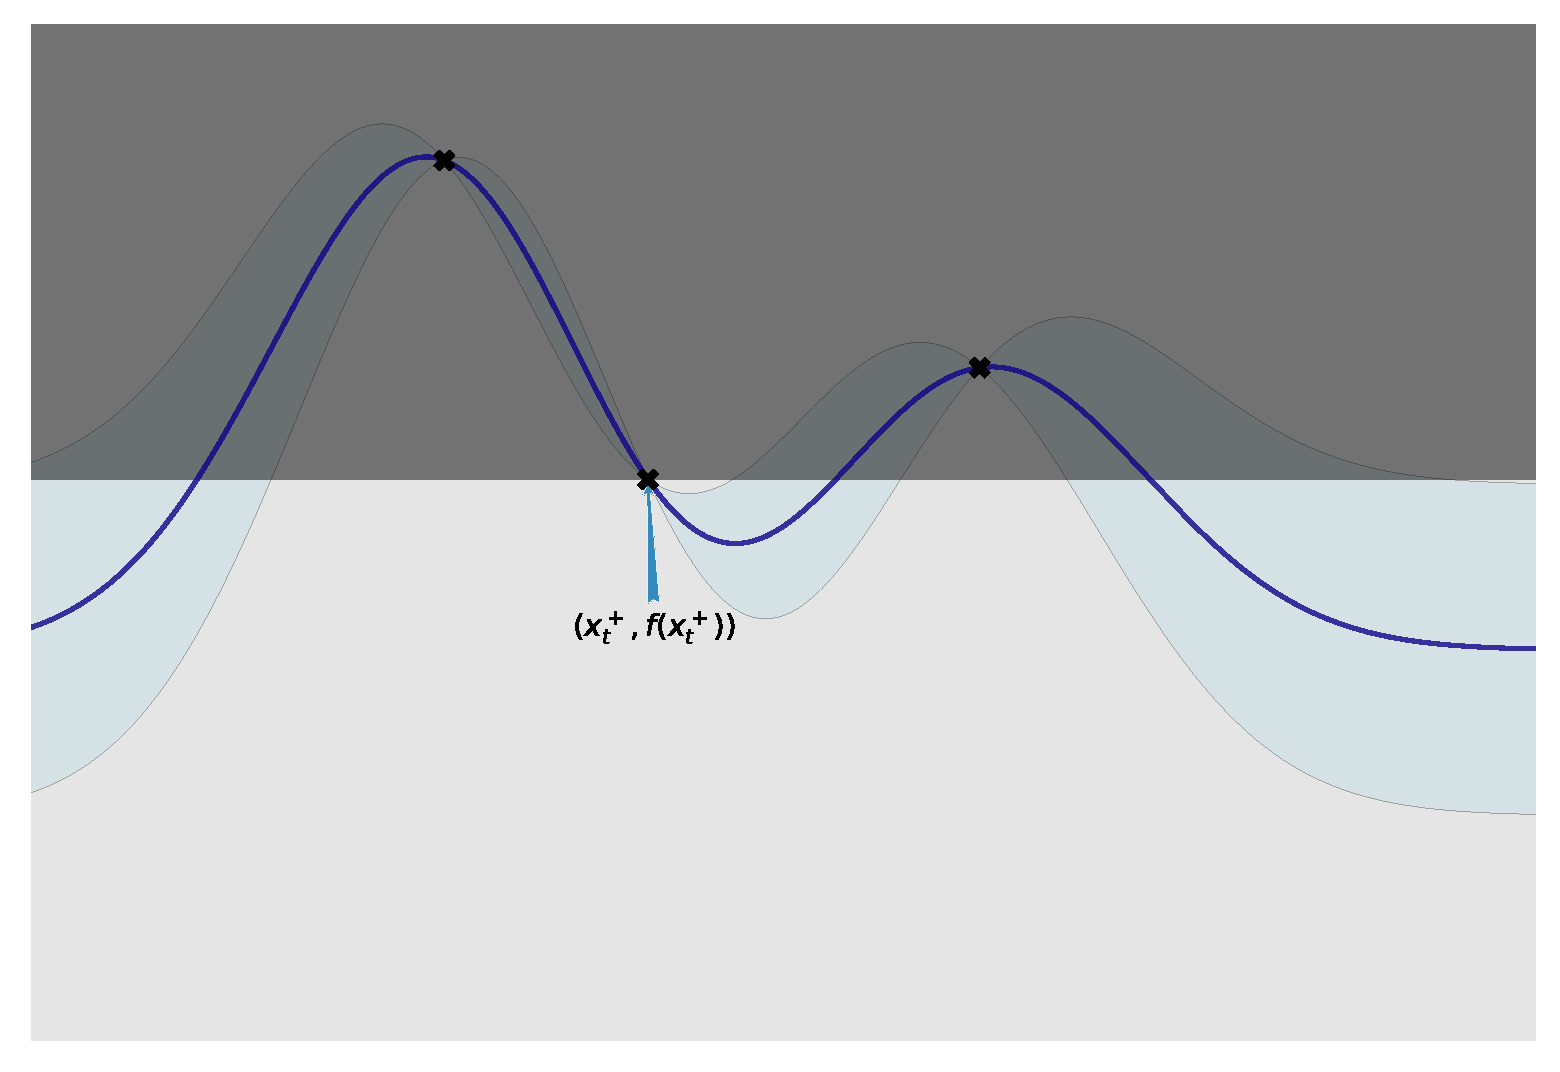
\includegraphics[width=.7\linewidth, height=0.7\textheight, keepaspectratio=true]{images/acq_func_images/pi_3.pdf}};
    \node<.> [below=0.01\belowcaptionskip of img3, align=center]{Region of probable improvement};

    \node<+> (img4) {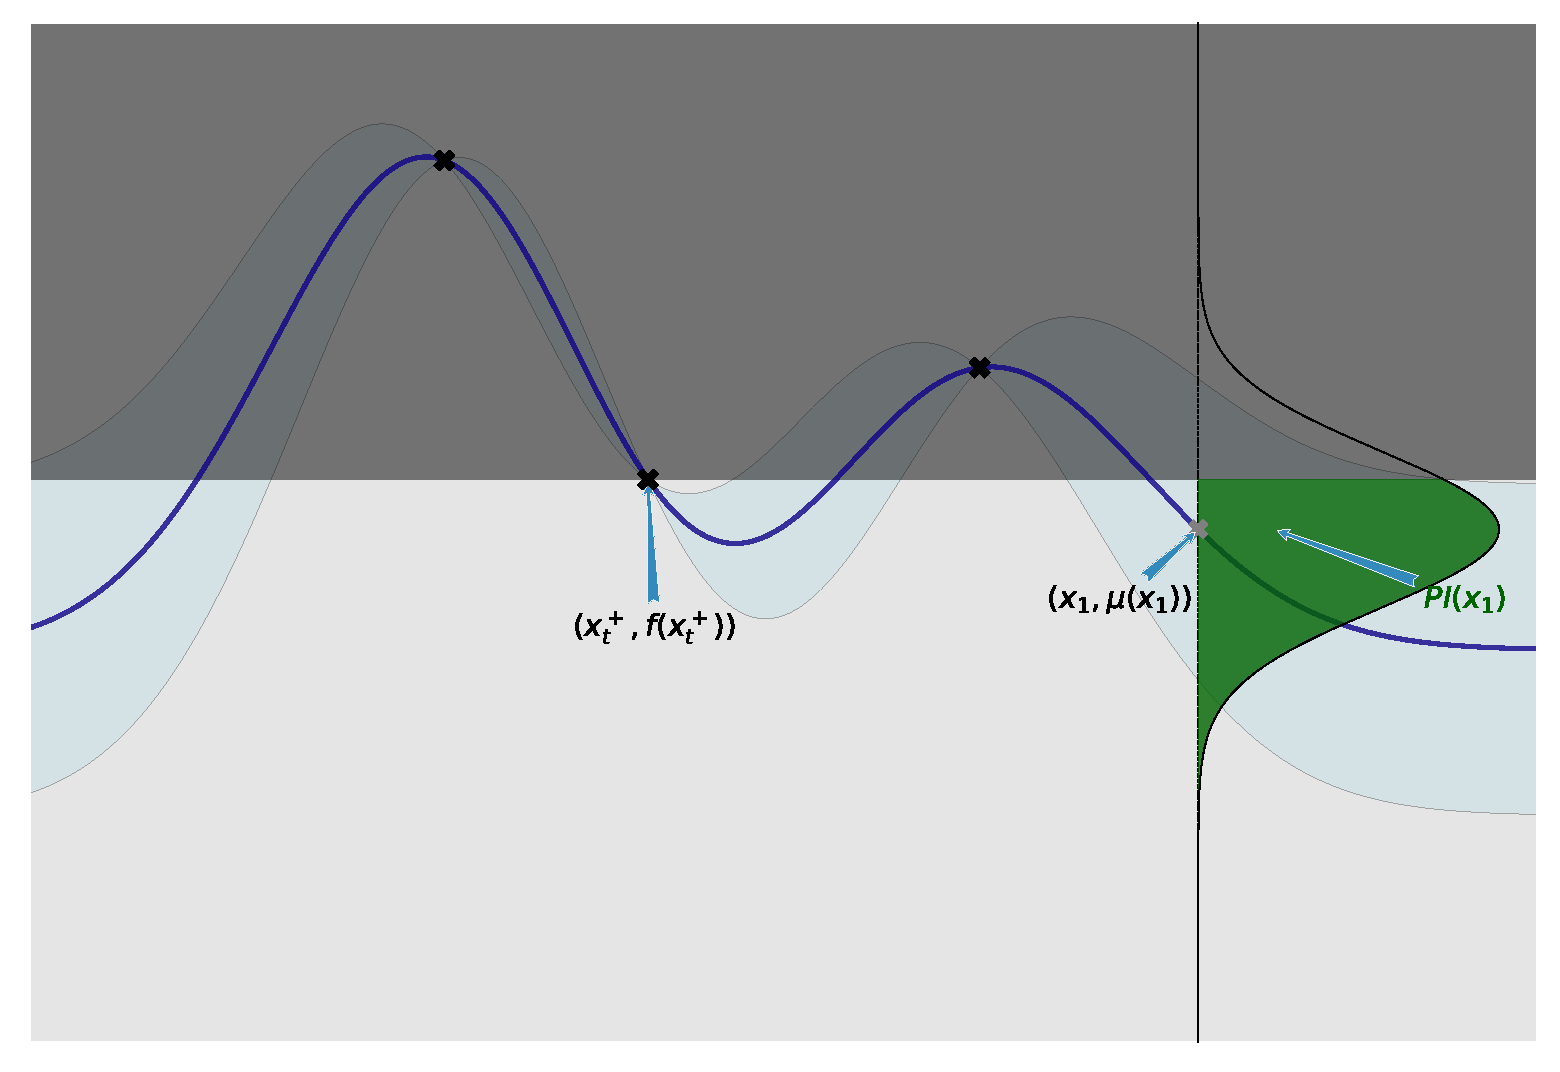
\includegraphics[width=.7\linewidth, height=0.7\textheight, keepaspectratio=true]{images/acq_func_images/pi_4.pdf}};
    \node<.> [below=0.01\belowcaptionskip of img4, align=center]{PDF of a good candidate parameter value};

    \node<+> (img5) {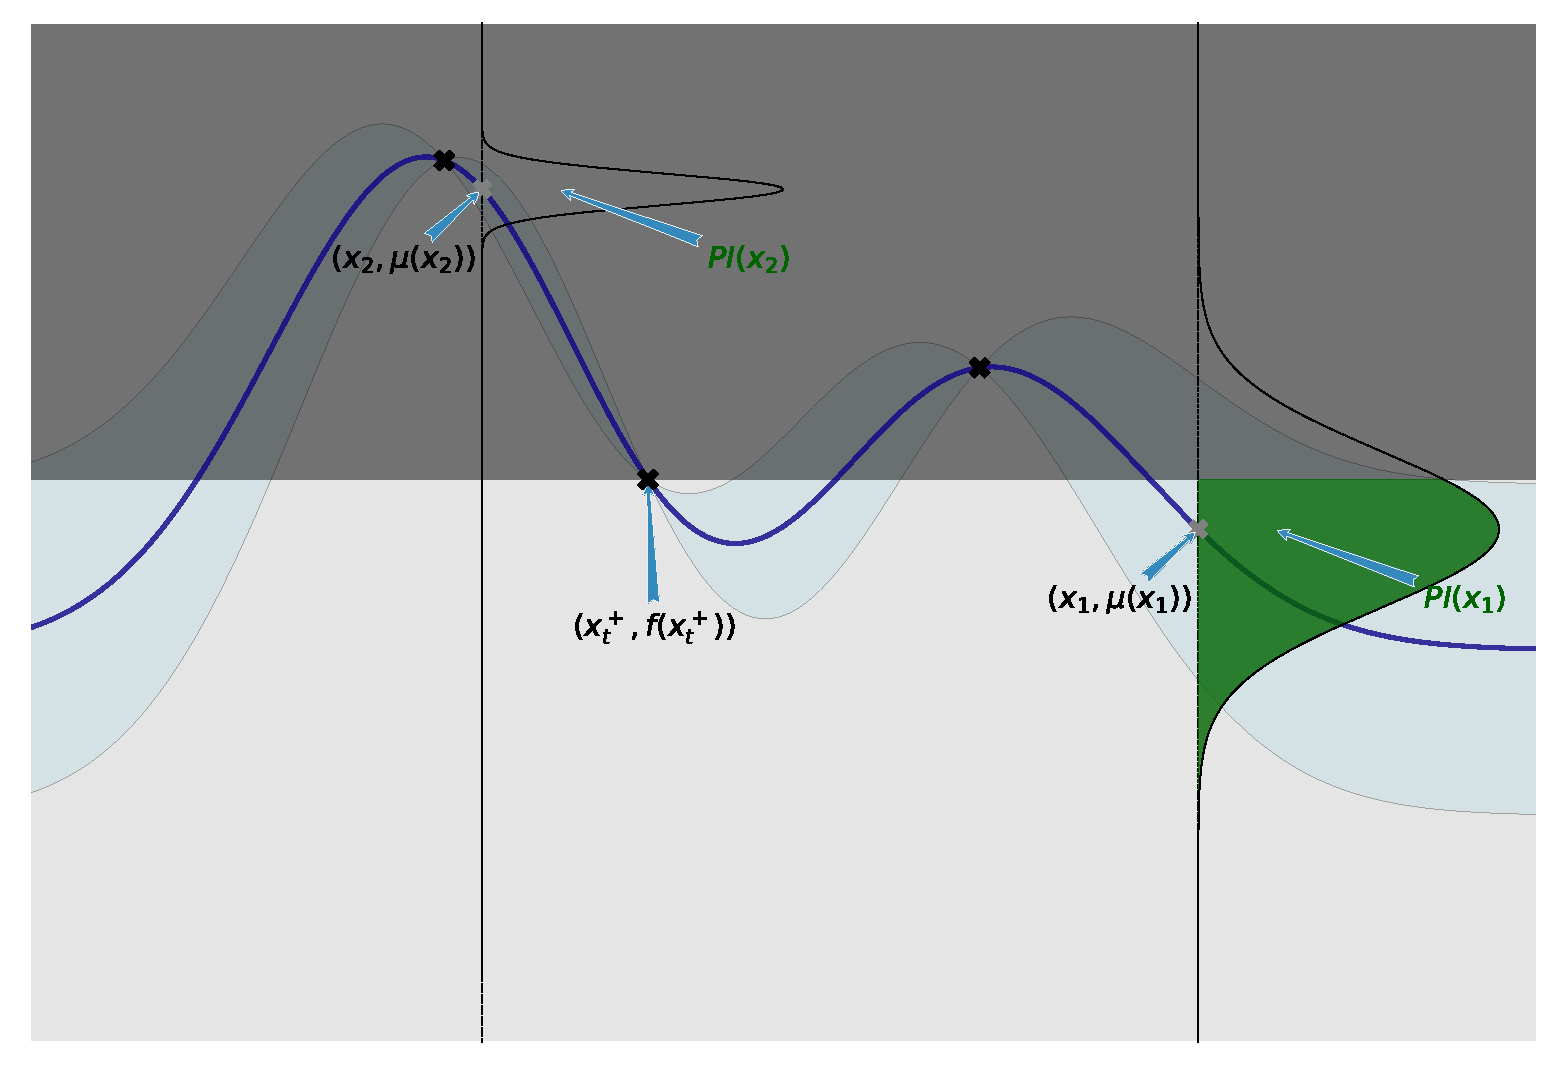
\includegraphics[width=.7\linewidth, height=0.7\textheight, keepaspectratio=true]{images/acq_func_images/pi_5.pdf}};
    \node<.> [below=0.01\belowcaptionskip of img5, align=center]{PDF of a bad candidate parameter value};
  \end{tikzpicture}
\end{figure}

\end{frame}
%-----------------------------------------------------------------------
\begin{frame}[c]{Basic Acquisition Functions - PI}
\framesubtitle{Probability of Improvement - Choosing a candidate}
\comment{Verify if definitions suit minimization!}
\begin{itemize}
    \item[]
        \[
            \iter{PI}(\conf) = P(\cost(\conf) \leq \cost(\incumbent[\bocount-1])), \quad \text{where } \incumbent[\bocount-1]\in\argmin_{\conf'\in\iter[\bocount-1]{\dataset}}\boobs\in\iter[\bocount-1]{\dataset}
        \]
\pause
\bigskip
\bigskip
This can be written as:
\vspace*{-1.0cm}
    \[
        \iter{PI}(\conf) = \cdf[Z], \quad \text{with } Z = \dfrac{\cost(\incumbent[\bocount-1]) - \iter[\bocount-1]{\mean}(\conf) - \xi}{\iter[\bocount-1]{\stddev}(\conf)}, 
    \]
    \newline
    where $\cdf(\cdot)$ is the CDF of the standard normal distribution and $\xi$ is an optional exploration parameter.
    \pause
    \item[] \[\boxed{\text{Choose } \bonextsample \in \argmax_{\conf\in\pcs}(\iter{PI}(\conf))}\]
%    \comment{Source: Tutorial by Brochu et al.: https://arxiv.org/pdf/1012.2599.pdf }
\end{itemize}
\end{frame}
%-----------------------------------------------------------------------
% \begin{frame}[c]{Basic Acquisition Functions - PI}
% \framesubtitle{Probability of Improvement - Features}
% \comment{To be replaced with a table of comparative features.}
% \begin{itemize}
%     \item Pure, greedy exploitation.
%     \item Intuitive.
%     \item Many known modes of failure.
% \end{itemize}
% \end{frame}
%-----------------------------------------------------------------------
\begin{frame}[c]{Basic Acquisition Functions - EI}
\framesubtitle{Expected Improvement - Concept}

\begin{figure}
  \centering
  \begin{tikzpicture}
    \node<+> (img1) {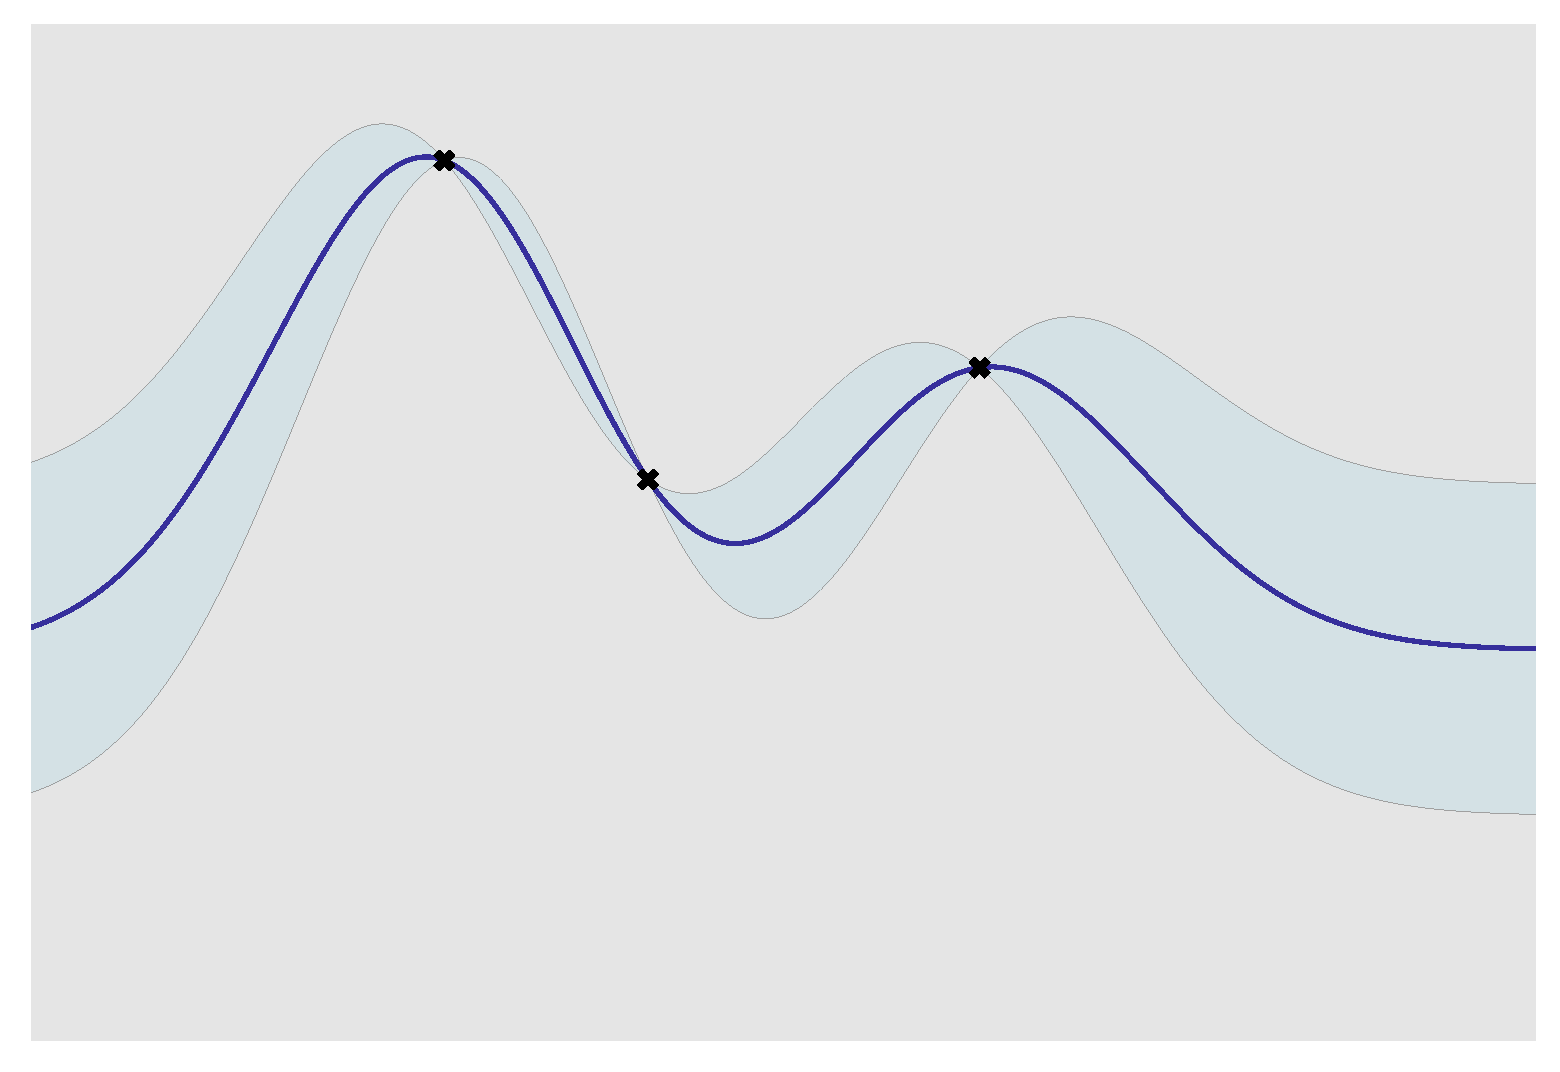
\includegraphics[width=.7\linewidth, height=0.7\textheight, keepaspectratio=true]{images/acq_func_images/ei_1.pdf}};
    \node<.> [below=0.01\belowcaptionskip of img1, align=center]{GP fit on 3 observations};

    \node<+> (img2) {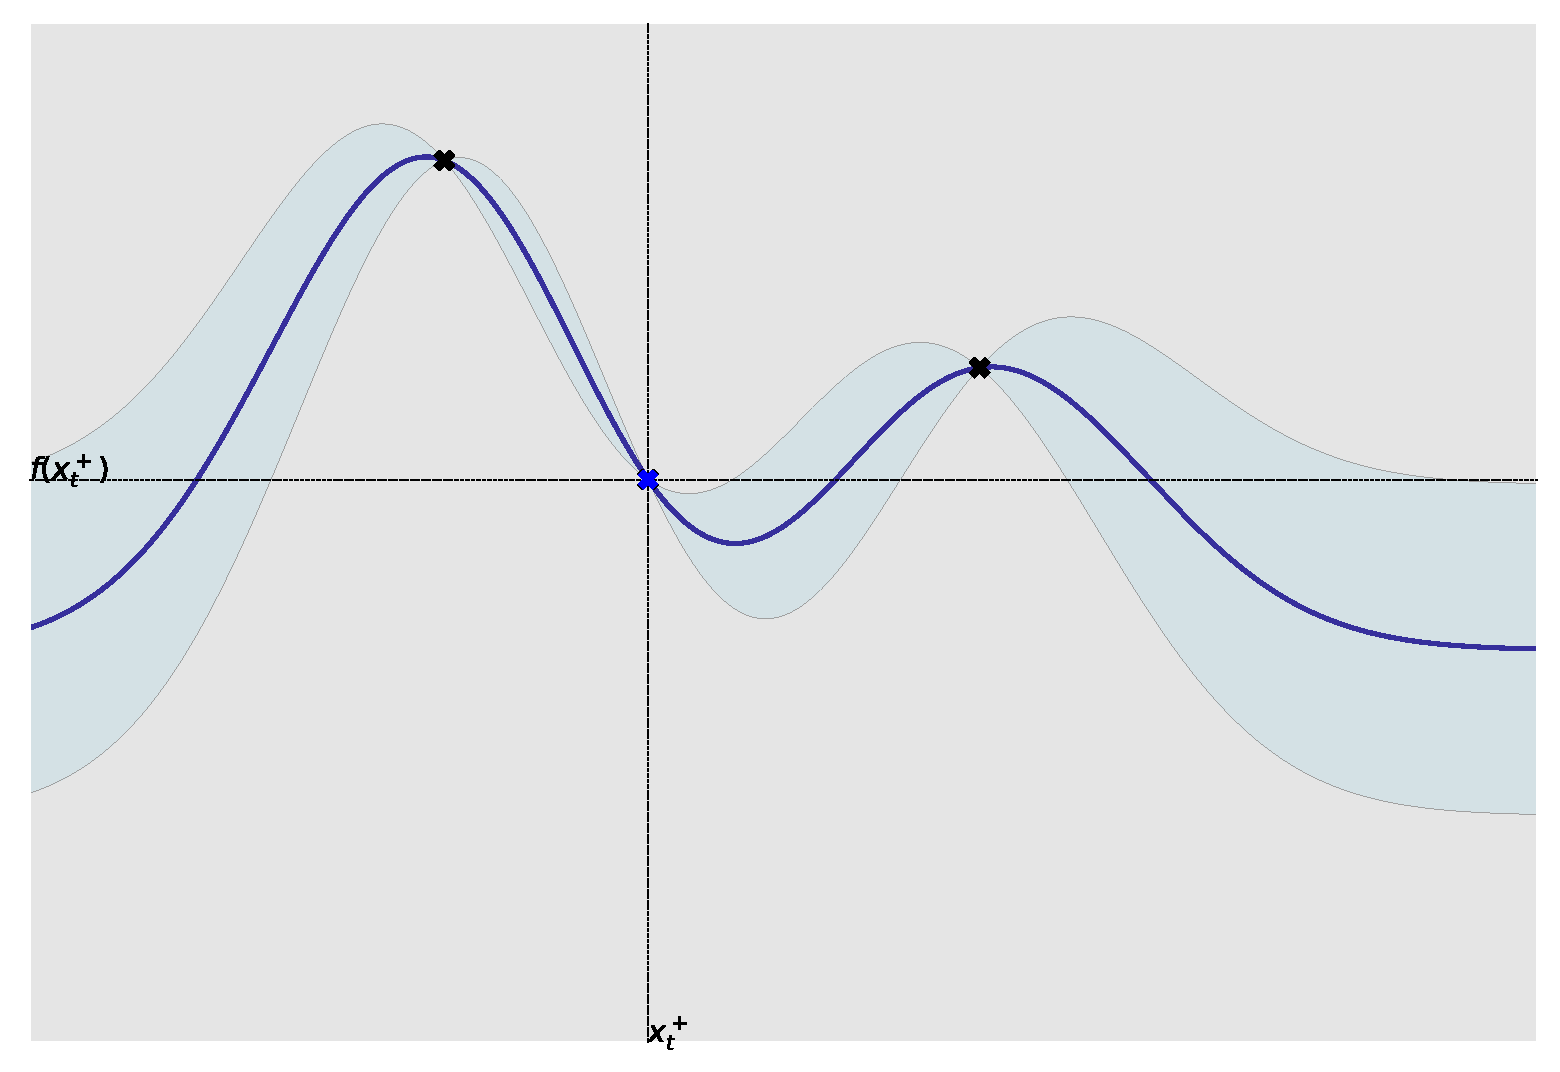
\includegraphics[width=.7\linewidth, height=0.7\textheight, keepaspectratio=true]{images/acq_func_images/ei_2.pdf}};
    \node<.> [below=0.01\belowcaptionskip of img2, align=center]{Current incumbent $\incumbent[\bocount-1]$ and its observed value $\cost(\incumbent[\bocount-1])$.};

    \node<+> (img3) {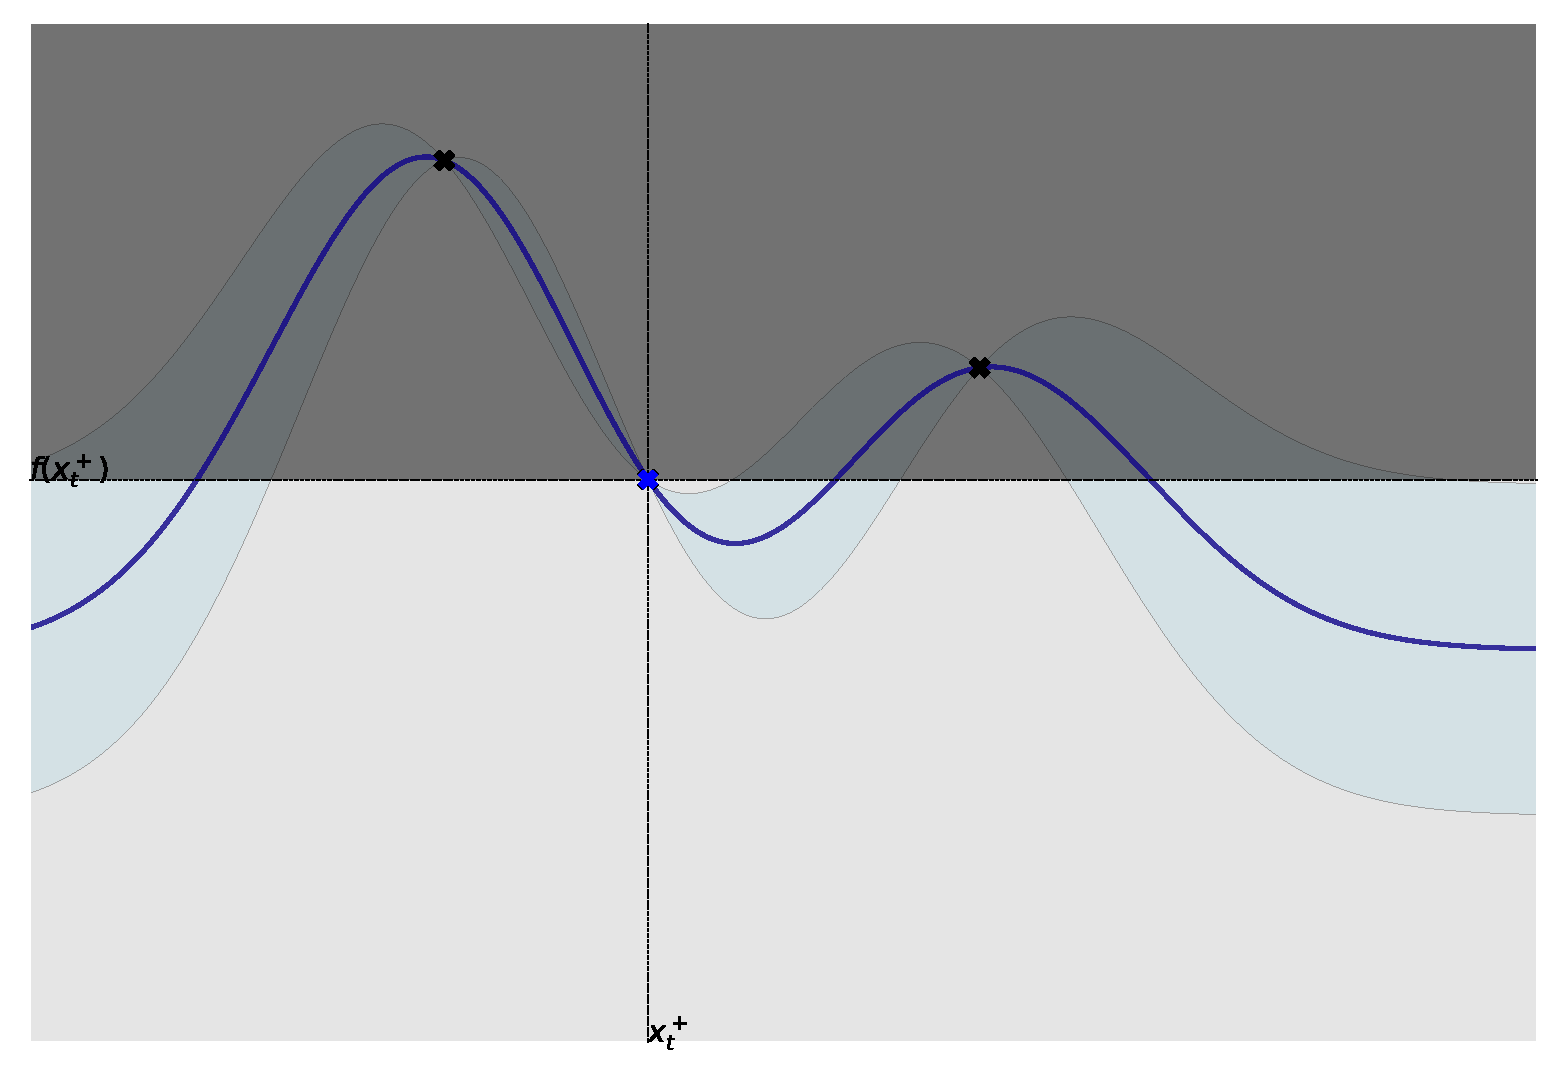
\includegraphics[width=.7\linewidth, height=0.7\textheight, keepaspectratio=true]{images/acq_func_images/ei_3.pdf}};
    \node<.> [below=0.01\belowcaptionskip of img3, align=center]{Zone of probable improvement};

    \node<+> (img4) {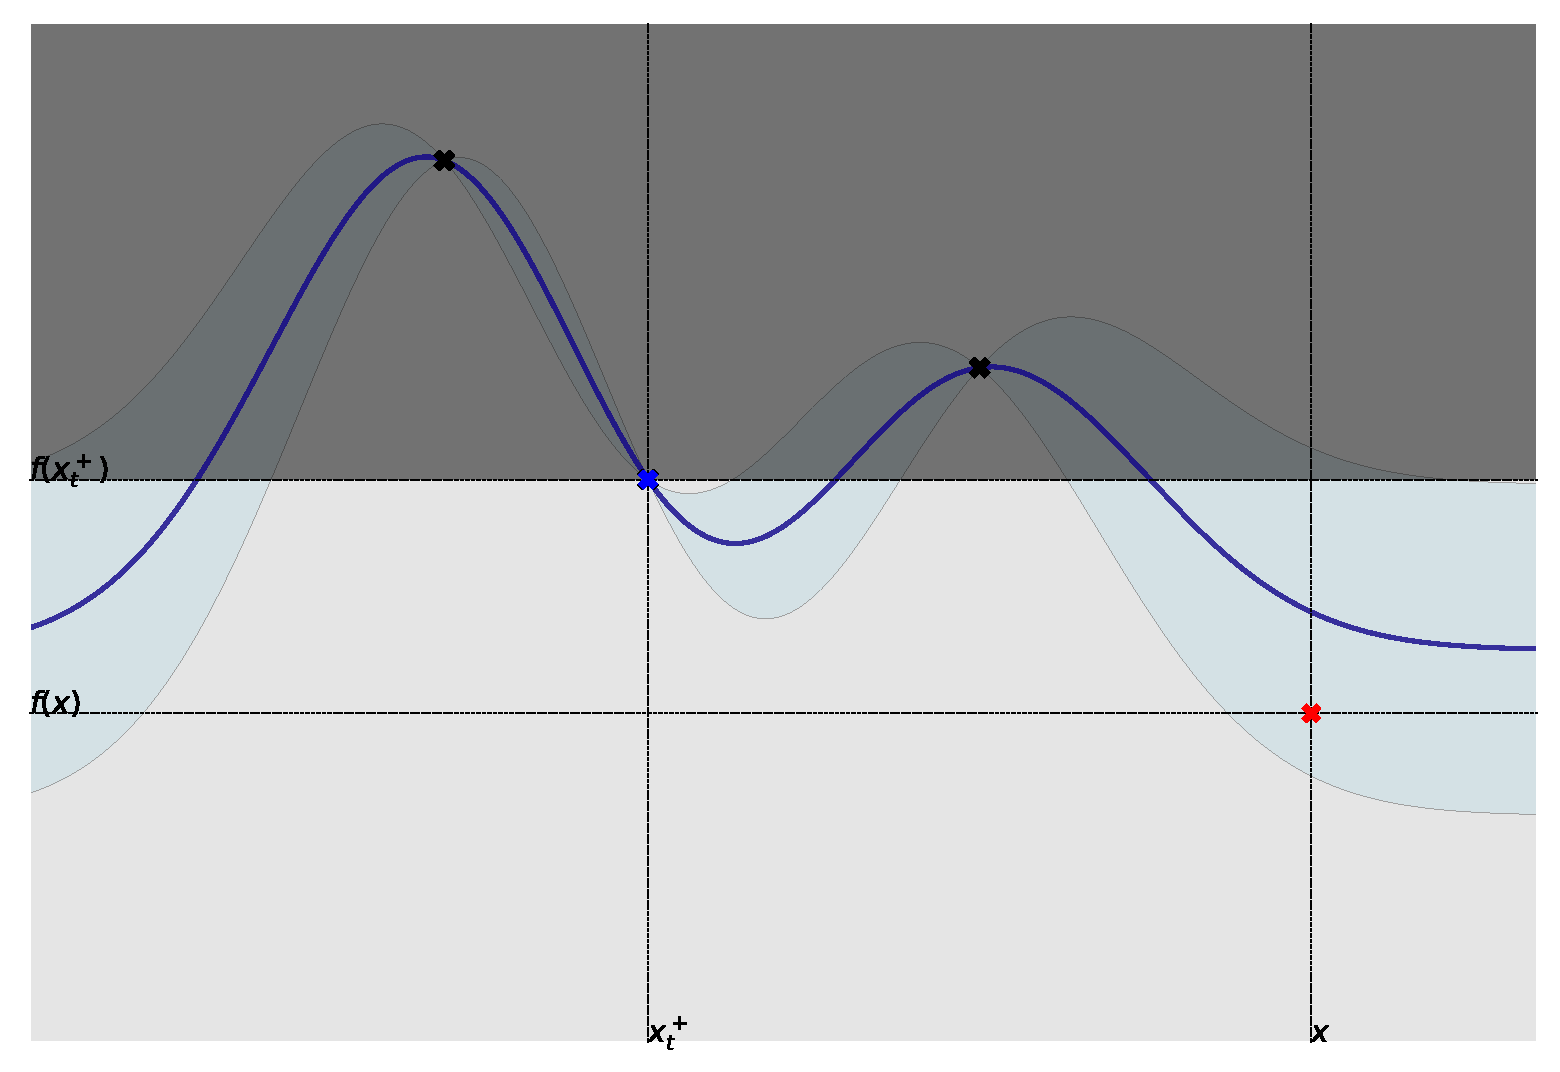
\includegraphics[width=.7\linewidth, height=0.7\textheight, keepaspectratio=true]{images/acq_func_images/ei_4.pdf}};
    \node<.> [below=0.01\belowcaptionskip of img4, align=center]{Hypothetical \emph{real} cost at a given $\conf$ - unknown in practice};

    \node<+> (img5) {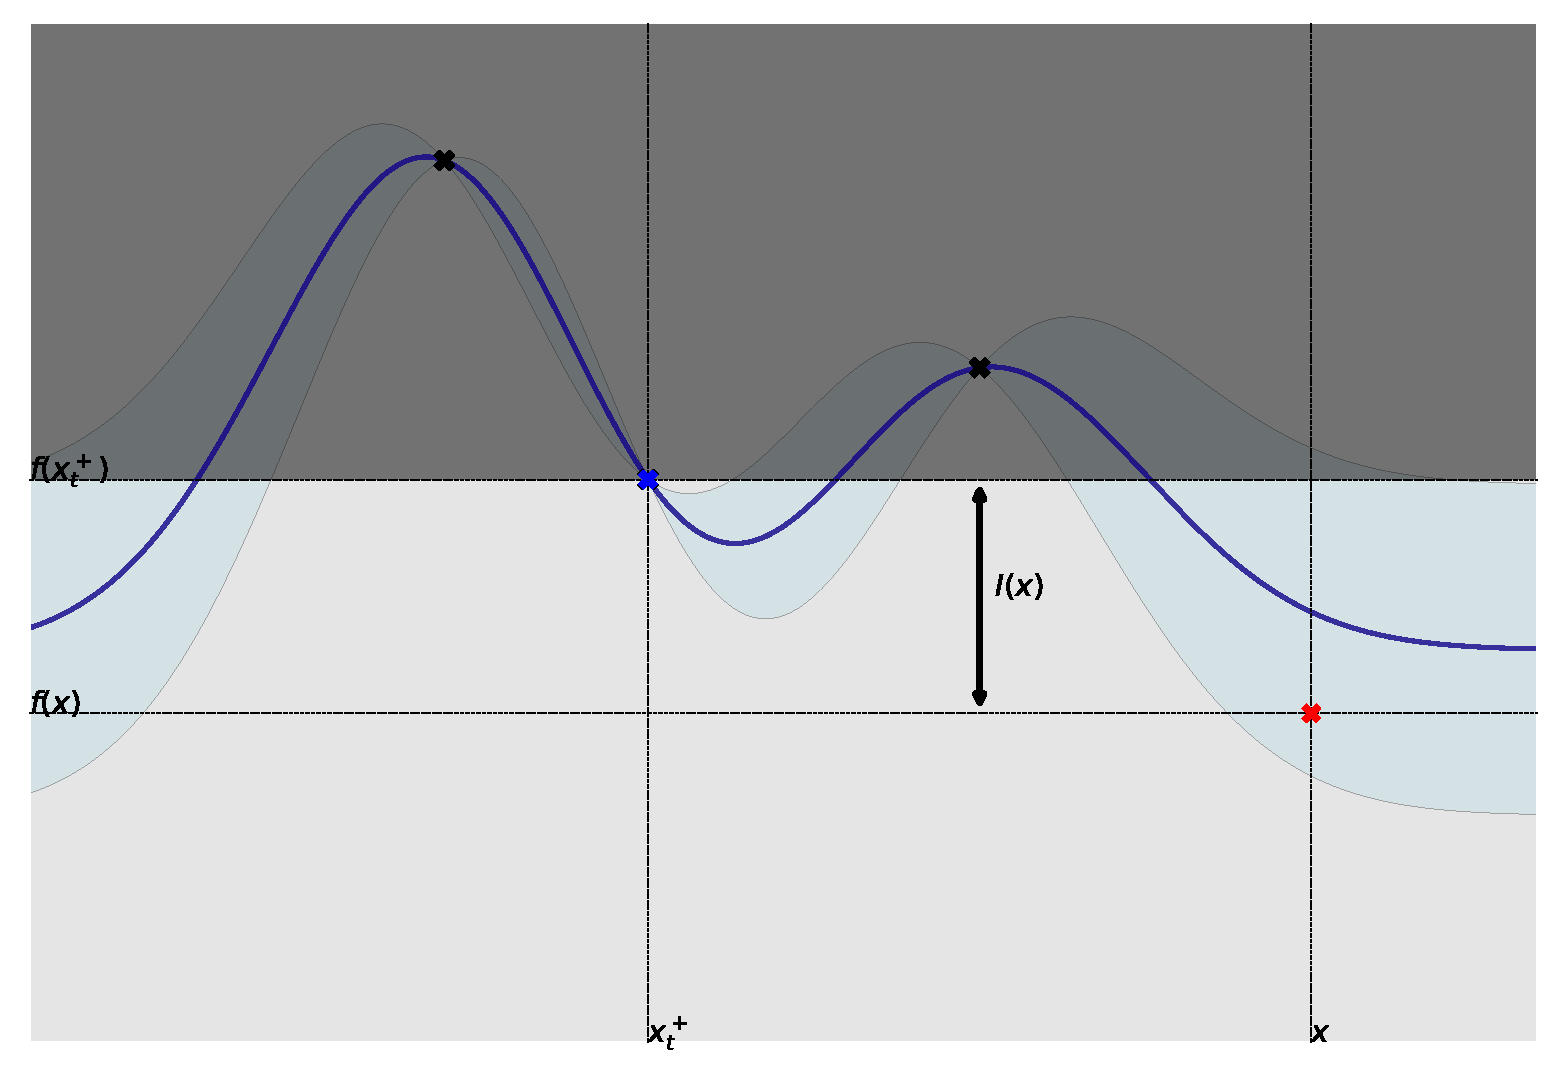
\includegraphics[width=.7\linewidth, height=0.7\textheight, keepaspectratio=true]{images/acq_func_images/ei_5.pdf}};
    \node<.> [below=0.01\belowcaptionskip of img4, align=center]{Actual improvement $I(\conf)$ - cannot be calculated before an evaluation!};

    \node<+> (img6) {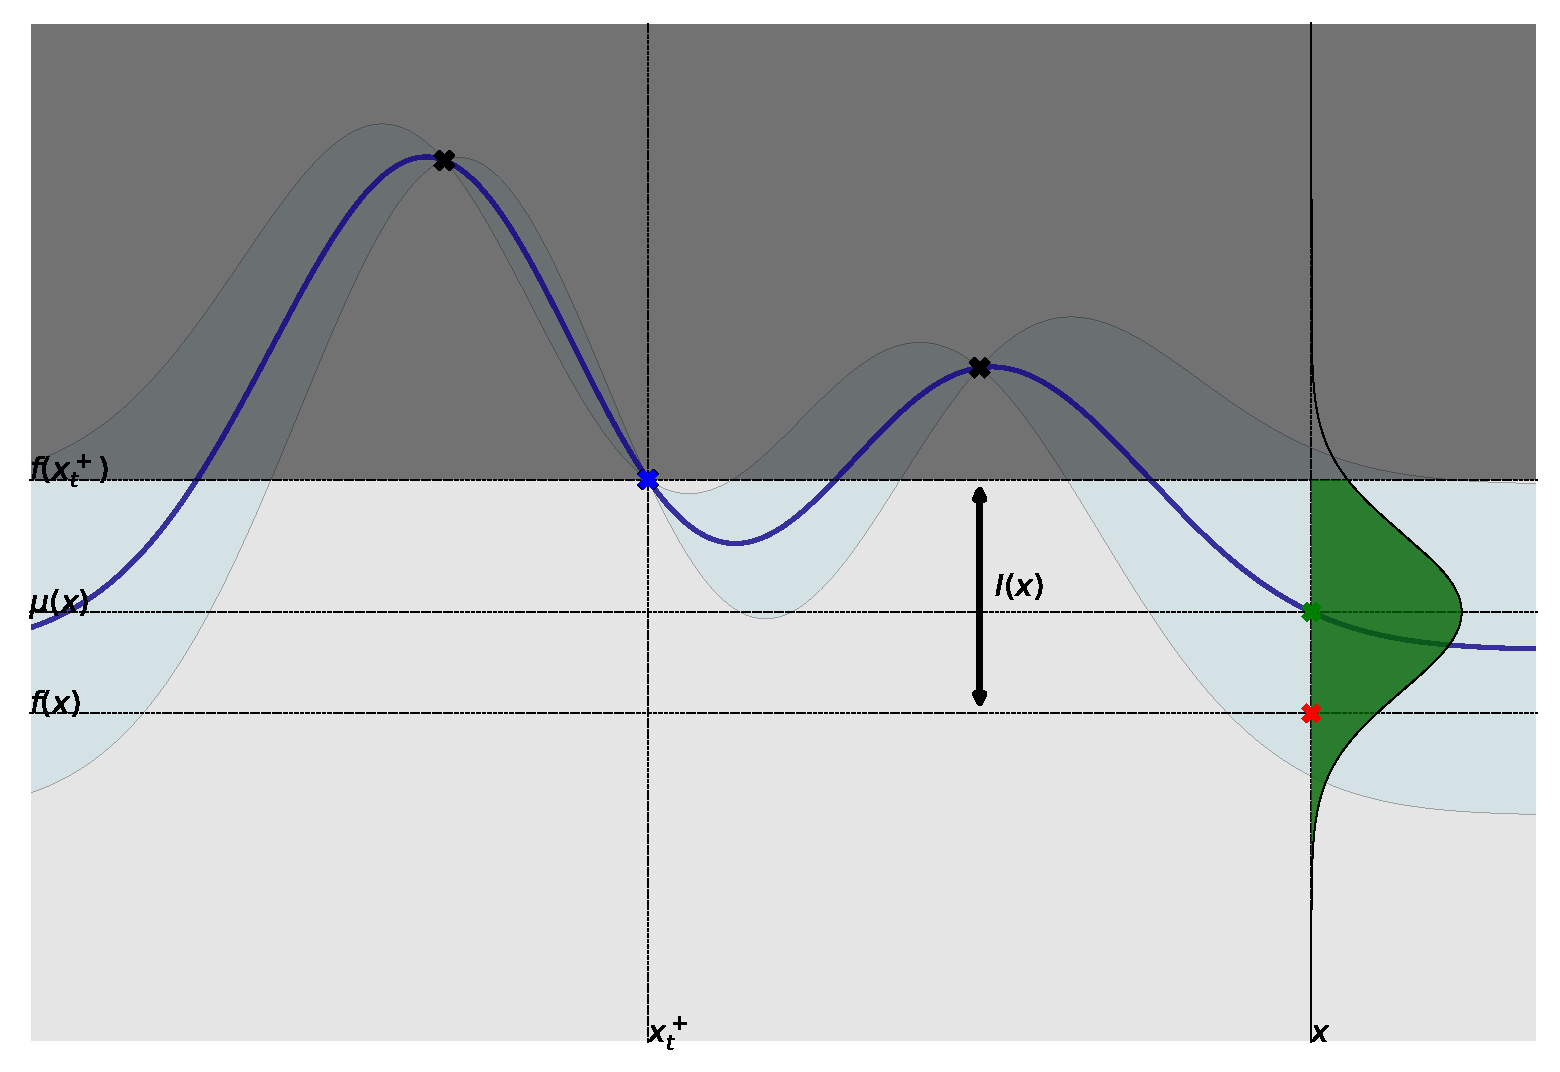
\includegraphics[width=.7\linewidth, height=0.7\textheight, keepaspectratio=true]{images/acq_func_images/ei_6.pdf}};
    \node<.> [below=-0.01\belowcaptionskip of img6, align=center]{$\E[\iter{\surro}(\conf)]$ - \emph{can} be calculated before an evaluation.};
    % \node<.> [below=-0.01\belowcaptionskip of img6, align=center]{$\E[\normaldist(\iter[\bocount-1]{\mean}(\conf), \iter[\bocount-1]{\left(\variance\right)}(\conf))]$ - \emph{can} be calculated before an evaluation.};

    \node<+> (img7) {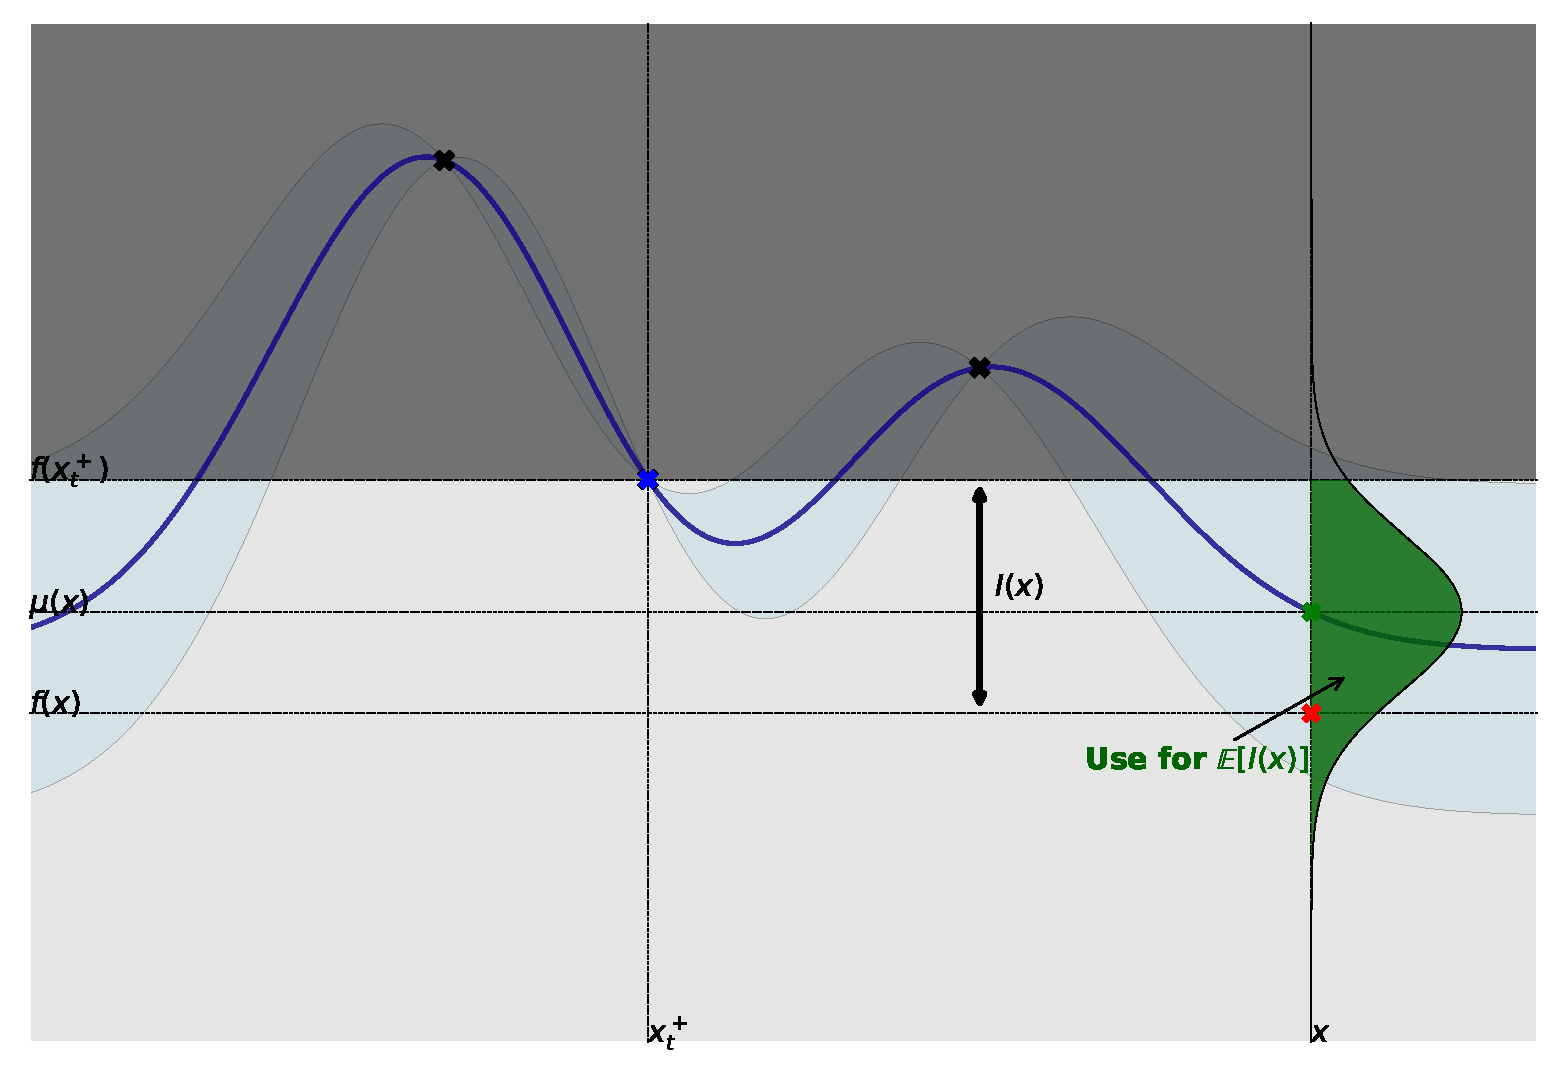
\includegraphics[width=.7\linewidth, height=0.7\textheight, keepaspectratio=true]{images/acq_func_images/ei_7.pdf}};
    \node<.> [below=0.01\belowcaptionskip of img7, align=center]{Use $\mean(\conf)$ and $\variance(\conf)$ to get $\E[I(\conf)]$};
  \end{tikzpicture}
\end{figure}

\end{frame}
%-----------------------------------------------------------------------
\begin{frame}[c]{Basic Acquisition Functions - EI}
\framesubtitle{Expected Improvement - Choosing a candidate}
\comment{Verify if formulae agree with minimizing the surrogate.}
\begin{itemize}\abovedisplayskip=0pt\belowdisplayskip=-0.5em
    \item[] We first define one-step improvement over the current incumbent, as
\smallskip
    \[
        \iter{I}(\conf) = \max(0, \cost(\incumbent[\bocount-1]) - \cost(\conf)), \quad\incumbent[\bocount-1]\in\argmax_{\conf'\in\iter[\bocount-1]{\dataset}}\boobs\in\iter[\bocount-1]{\dataset}
    \]
\pause
\medskip
    \item[] Expected Improvement is then defined as
    \begin{align*}
        \iter{EI}(\conf) &= \E[\iter{I}(\conf)]\\
        &= \int_{\iter{I}=0}^{\iter{I}=\infty}\iter{I} P(\iter{I})d\iter{I}
    \end{align*}
\pause
\medskip
    \item[]If we use a normal distribution as the probability for $\iter{I}$,
    \[
        P(\iter{I}) =
            \dfrac{1}{\sqrt{2\pi}\iter{\stddev}(\conf)}\exp{-\dfrac{{(\cost(\incumbent[\bocount-1])-\iter{\mean}(\conf)-\iter{I})}^2}{2\iter{\left(\variance\right)}(\conf)}
        }
    \]
\end{itemize}
\end{frame}
%-----------------------------------------------------------------------
% \begin{frame}[c]{Basic Acquisition Functions - EI}
% \framesubtitle{Expected Improvement - Choosing a candidate}
%     \begin{align*}
%         \action<+->{\iter{EI}(\conf) &= \int_{\iter{I}=0}^{\iter{I}=\infty}\iter{I} \dfrac{1}{\sqrt{2\pi}\iter{\stddev}(\conf)}\exp{-\dfrac{{(\cost(\incumbent[\bocount-1])-\iter{\mean}(\conf)-\iter{I})}^2}{2\iter{\left(\variance\right)}(\conf)}}d\iter{I}\\}
%         \action<+->{&= 
%             \begin{cases}
%                 (\cost(\incumbent) - \iter{\mean}(\conf) - \xi)\cdf(Z) + \iter{\stddev}(\conf) \pdf(Z), & \text{if }\iter{\stddev}(\conf) > 0 \\
%                 0 & \text{if }\iter{\stddev}(\conf) = 0
%             \end{cases}\\}
%         \action<+->{\intertext{where }Z} \action<.->{&=\dfrac{\cost(\incumbent) - \iter{\mean}(\conf) - \xi}{\iter{\stddev}(\conf)}}
%     \action<+->{\Aboxed{\bonextsample \in \argmax_{\conf\in\pcs}(\iter{EI}(\conf))}}
%     \end{align*}
% %    \comment{Source: Tutorial by Brochu et al.: https://arxiv.org/pdf/1012.2599.pdf }
% \end{frame}
%-----------------------------------------------------------------------
\begin{frame}[c]{Basic Acquisition Functions - EI}
\framesubtitle{Expected Improvement - Choosing a candidate}
%     \comment{Consider this alternative formulation of EI for the previous slide.}
    \begin{align*}
        \action<+->{\iter{EI}(\conf) &= \int_{\iter{I}=0}^{\iter{I}=\infty}\iter{I} \dfrac{1}{\sqrt{2\pi}\iter{\stddev}(\conf)}\exp{-\dfrac{{(\cost(\incumbent[\bocount-1])-\iter{\mean}(\conf)-\iter{I})}^2}{2\iter{\left(\variance\right)}(\conf)}}d\iter{I}\\}
        \action<+->{&= 
            \begin{cases}
                \iter{\stddev}(\conf)[Z\cdf(Z) + \pdf(Z)], & \text{if }\iter{\stddev}(\conf) > 0 \\
                0 & \text{if }\iter{\stddev}(\conf) = 0
            \end{cases}\\
        \intertext{where }Z &=\dfrac{\cost(\incumbent[\bocount-1]) - \iter{\mean}(\conf) - \xi}{\iter{\stddev}(\conf)}}
    \action<+->{\Aboxed{\text{Choose } \bonextsample \in \argmax_{\conf\in\pcs}(\iter{EI}(\conf))}}
    \end{align*}
%    \comment{Source: Tutorial by Brochu et al.: https://arxiv.org/pdf/1012.2599.pdf }
\end{frame}
%-----------------------------------------------------------------------
% \begin{frame}[c]{Basic Acquisition Functions - EI}
% \framesubtitle{Expected Improvement - Features}
% \comment{Replace with table of comparisons}
% \begin{itemize}
%     \item Enables an exploration-exploitation trade-off.
%     \item Analytical solutions for the multi-step setting exist.
%     \item One of the most commonly used acquisition functions.
% \end{itemize}
% \end{frame}
%-----------------------------------------------------------------------
\begin{frame}[c]{Basic Acquisition Functions - LCB/UCB}
\framesubtitle{Confidence Bounds - Concept}

\begin{figure}
  \centering
  \begin{tikzpicture}
    \node<+> (img1) {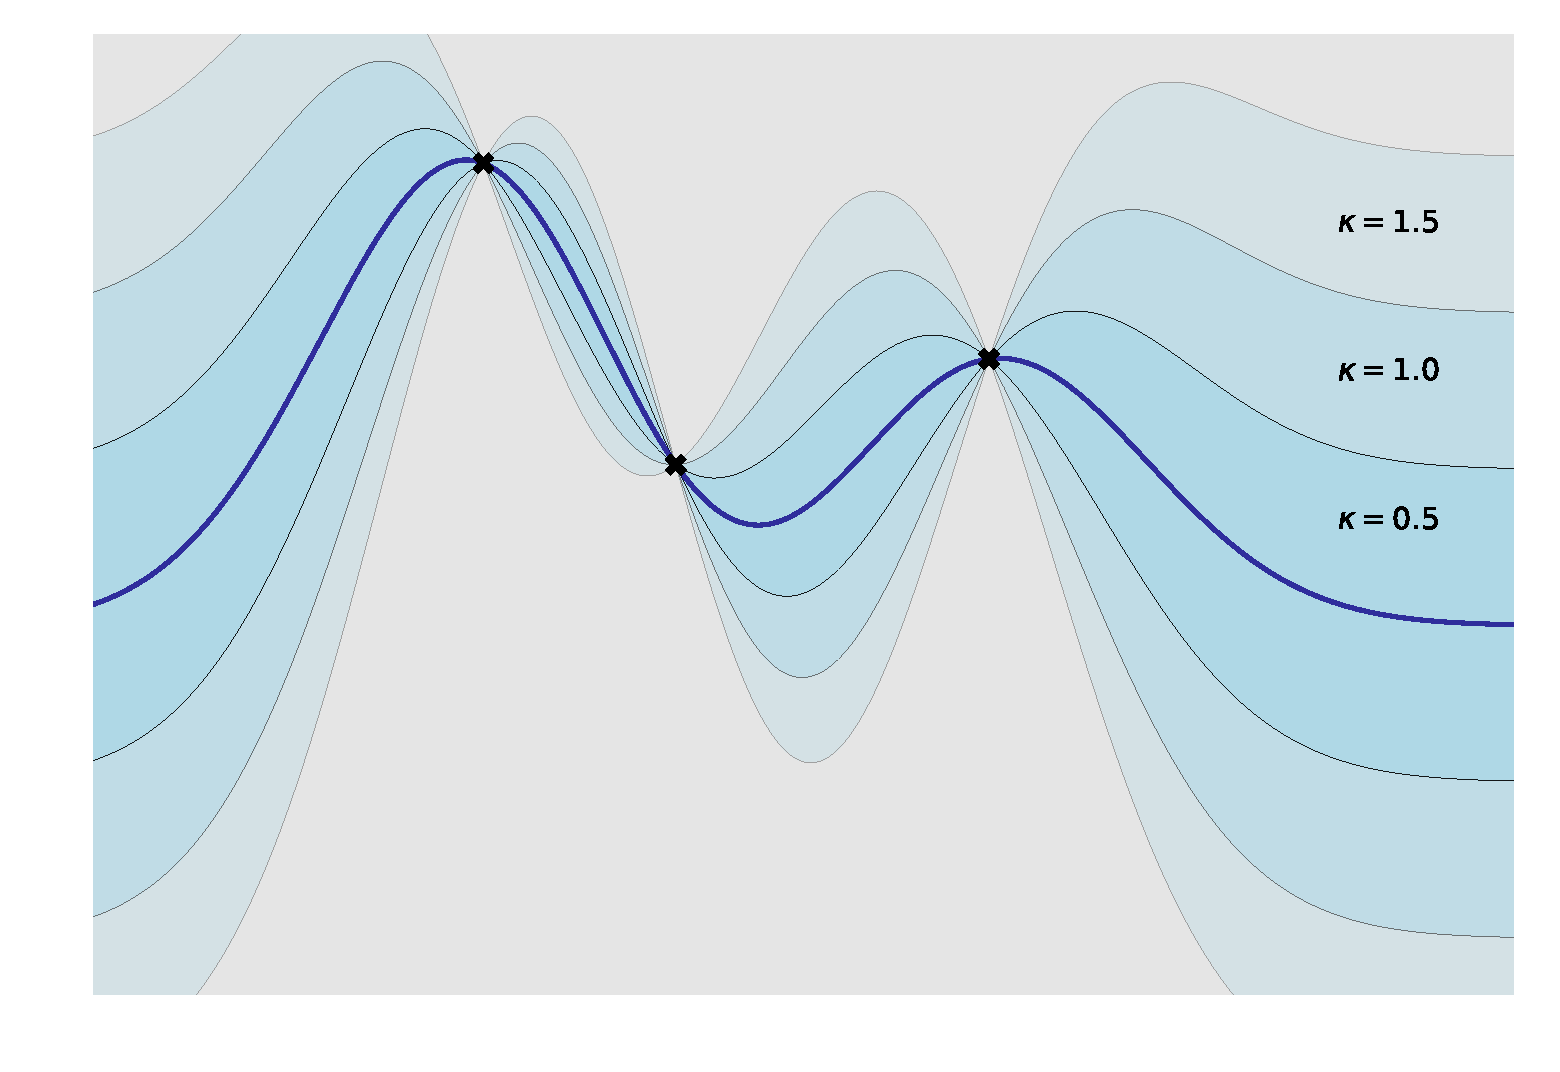
\includegraphics[width=.7\linewidth, height=0.7\textheight, keepaspectratio=true]{images/acq_func_images/lcb_1.pdf}};
    \node<.> [below=0.01\belowcaptionskip of img1, align=center]{Confidence Bound, $\mean(\conf)\pm\alpha\stddev(\conf)$};
    \node<+> (img2) {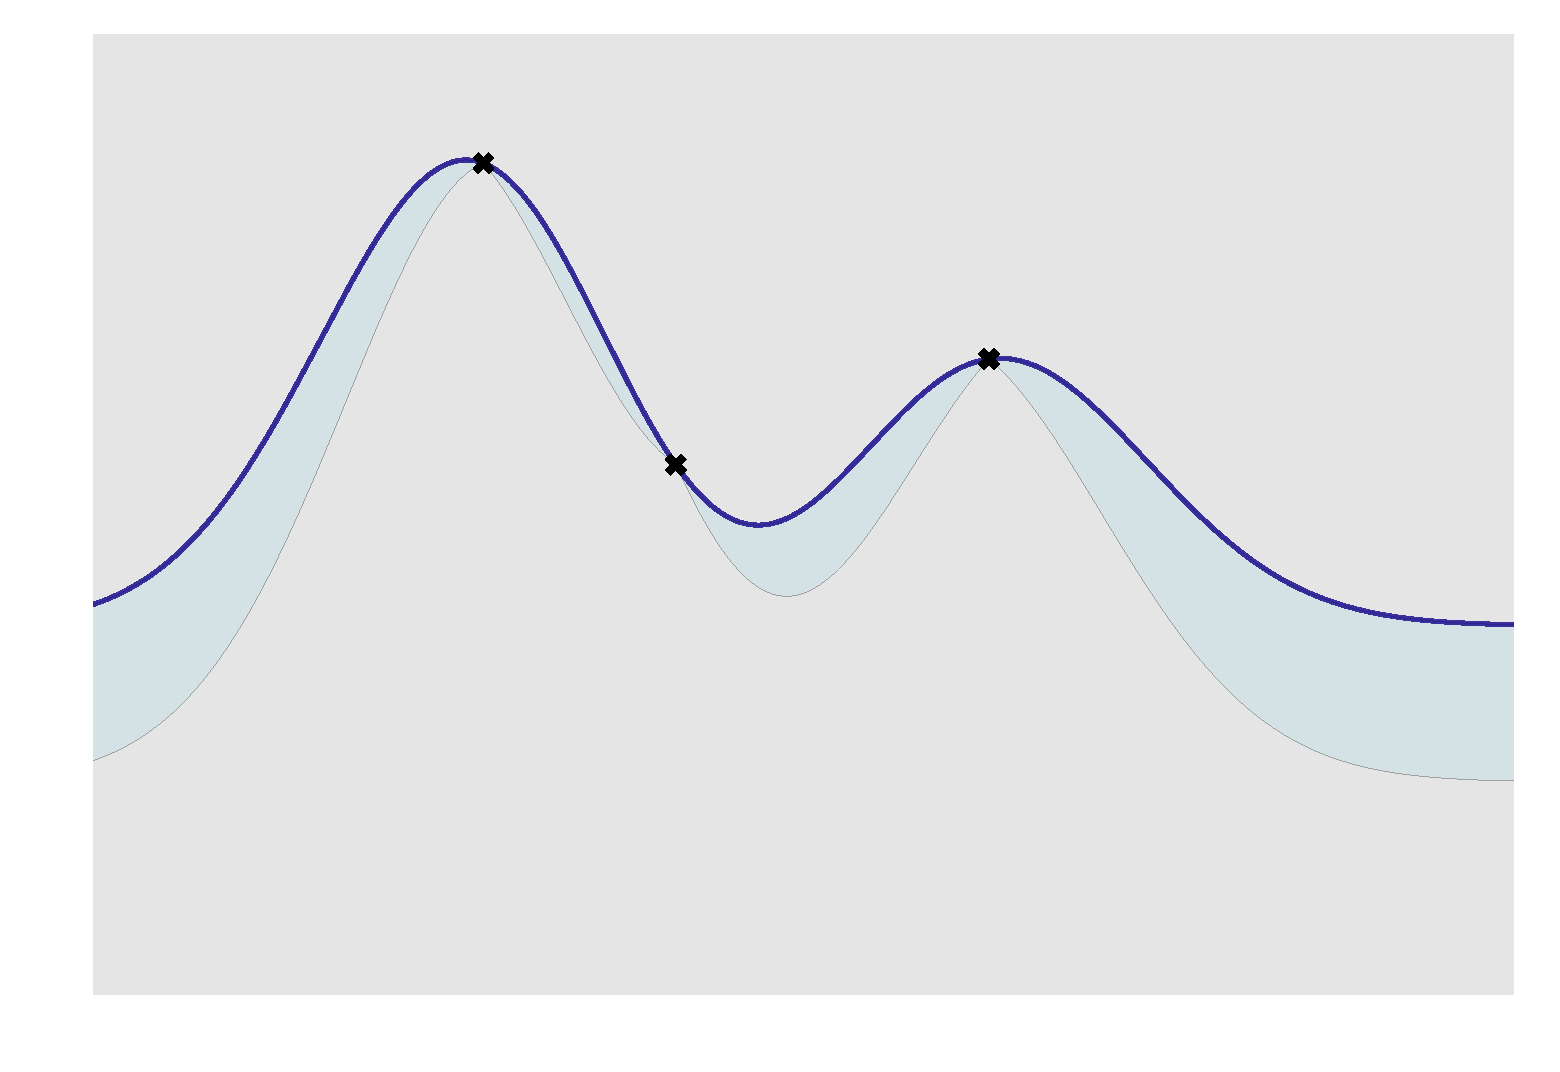
\includegraphics[width=.7\linewidth, height=0.7\textheight, keepaspectratio=true]{images/acq_func_images/lcb_2.pdf}};
    \node<.> [below=0.01\belowcaptionskip of img2, align=center]{Lower Confidence Bound, $\mean(\conf)-\alpha\stddev(\conf)$.};
    \node<+> (img3) {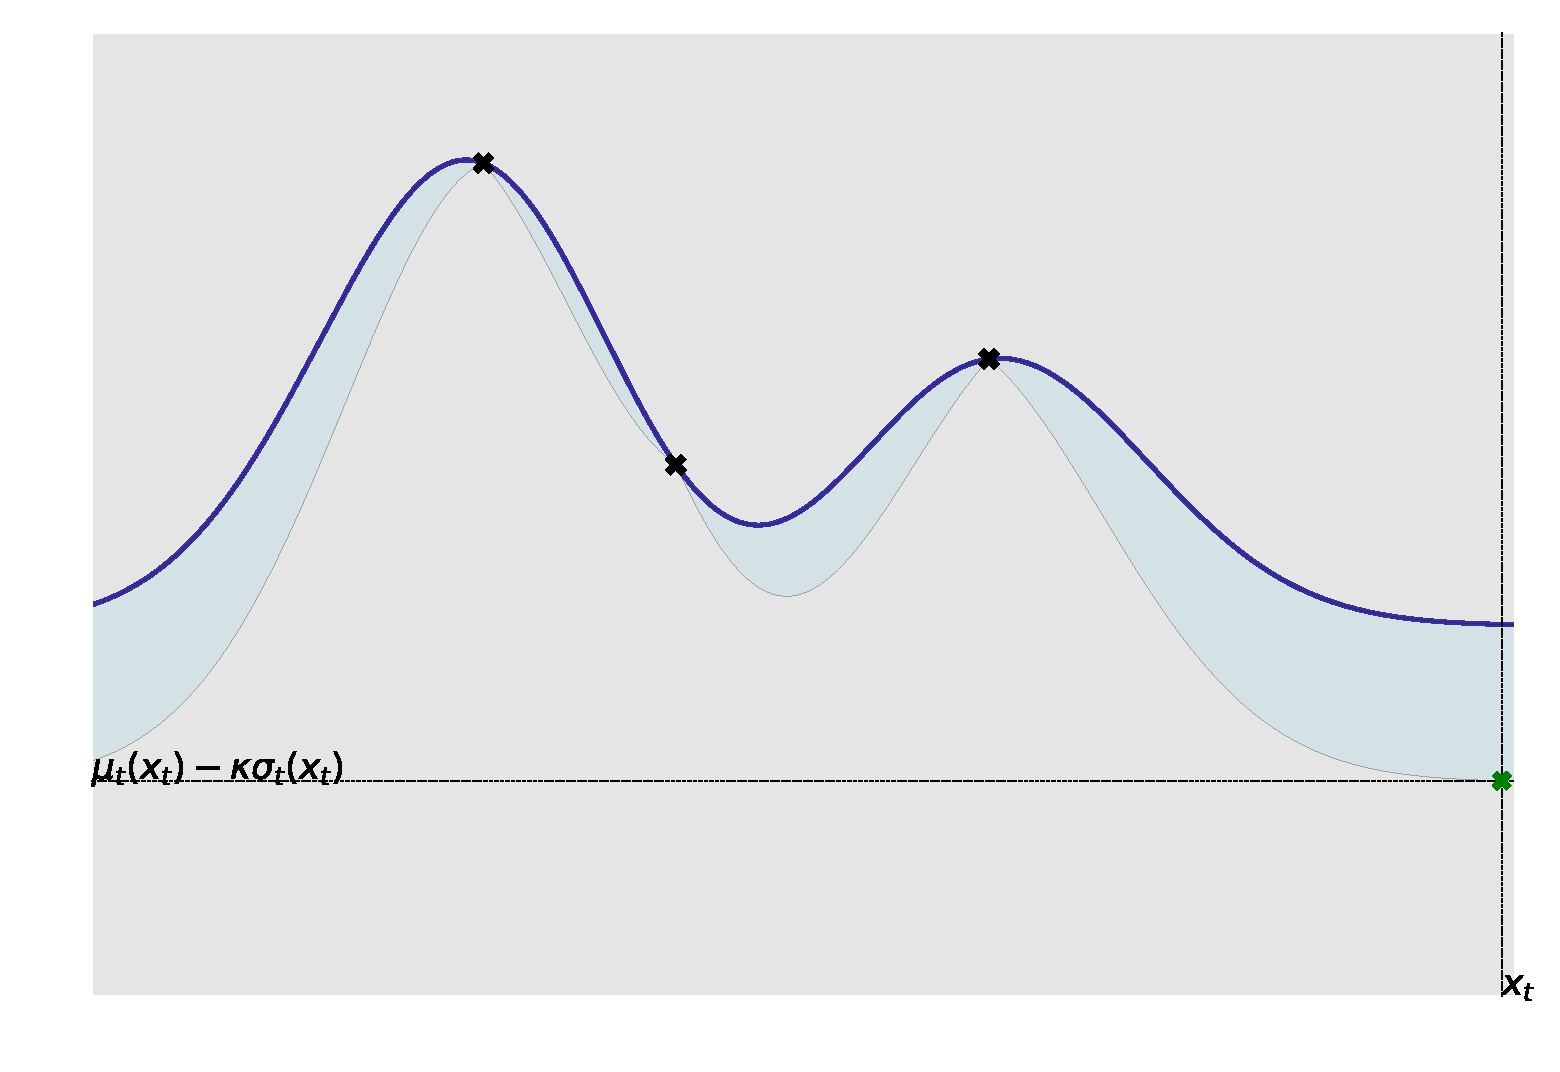
\includegraphics[width=.7\linewidth, height=0.7\textheight, keepaspectratio=true]{images/acq_func_images/lcb_3.pdf}};
    \node<.> [below=0.01\belowcaptionskip of img3, align=center]{To minimize cumulative regret, $\bonextsample=\argmin(LCB(\conf))$\comment{Verify!}};
  \end{tikzpicture}
\end{figure}

\end{frame}
%-----------------------------------------------------------------------
\begin{frame}[c]{Basic Acquisition Functions - LCB/UCB}
\framesubtitle{Confidence Bounds - Choosing a candidate}
\begin{itemize}
    \item<+->{We define the Lower Confidence Bound as 
    \[\iter{LCB}(\conf) = \iter{\mean}(\conf) - \alpha\iter{\stddev}(\conf),\quad\alpha\geq0\]}
    \item<+->{In the case of GPs, we define GP-LCB as
    \[\iter{GP-LCB}(\conf) = \iter{\mean}(\conf) - \sqrt{\nu\tau_t}\iter{\stddev}(\conf), \quad\nu>0\]}
    \item<+->{LCB is used to minimize cumulative regret.} 
    \item<+->{Question: When would you use Upper Confidence Bound (UCB) instead?}
    \comment{Source: Tutorial by Brochu et al.: https://arxiv.org/pdf/1012.2599.pdf }
\end{itemize}
\end{frame}
%-----------------------------------------------------------------------
% \begin{frame}[c]{Basic Acquisition Functions - LCB/UCB}
% \framesubtitle{Confidence Bounds - Features}
% \comment{Replace with table of comparisons}
% \begin{itemize}
%     \item Conceptually simple and easy to understand.
%     \item Inherently minimizes cumulative regret, or maximizes total reward.
%     \item Known theoretical guarantees under certain conditions for convergence.
%     \item Heavily dependent on the optimization of its hyperparameters - $\kappa$ in the general case, and $\nu$ and $\tau$ for the GP case.
% \end{itemize}
% \end{frame}
%-----------------------------------------------------------------------
\begin{frame}[c]{Basic Acquisition Functions - TS}
\framesubtitle{Thompson Sampling - Concept}

\begin{figure}
  \centering
  \begin{tikzpicture}
    \node<+> (img1) {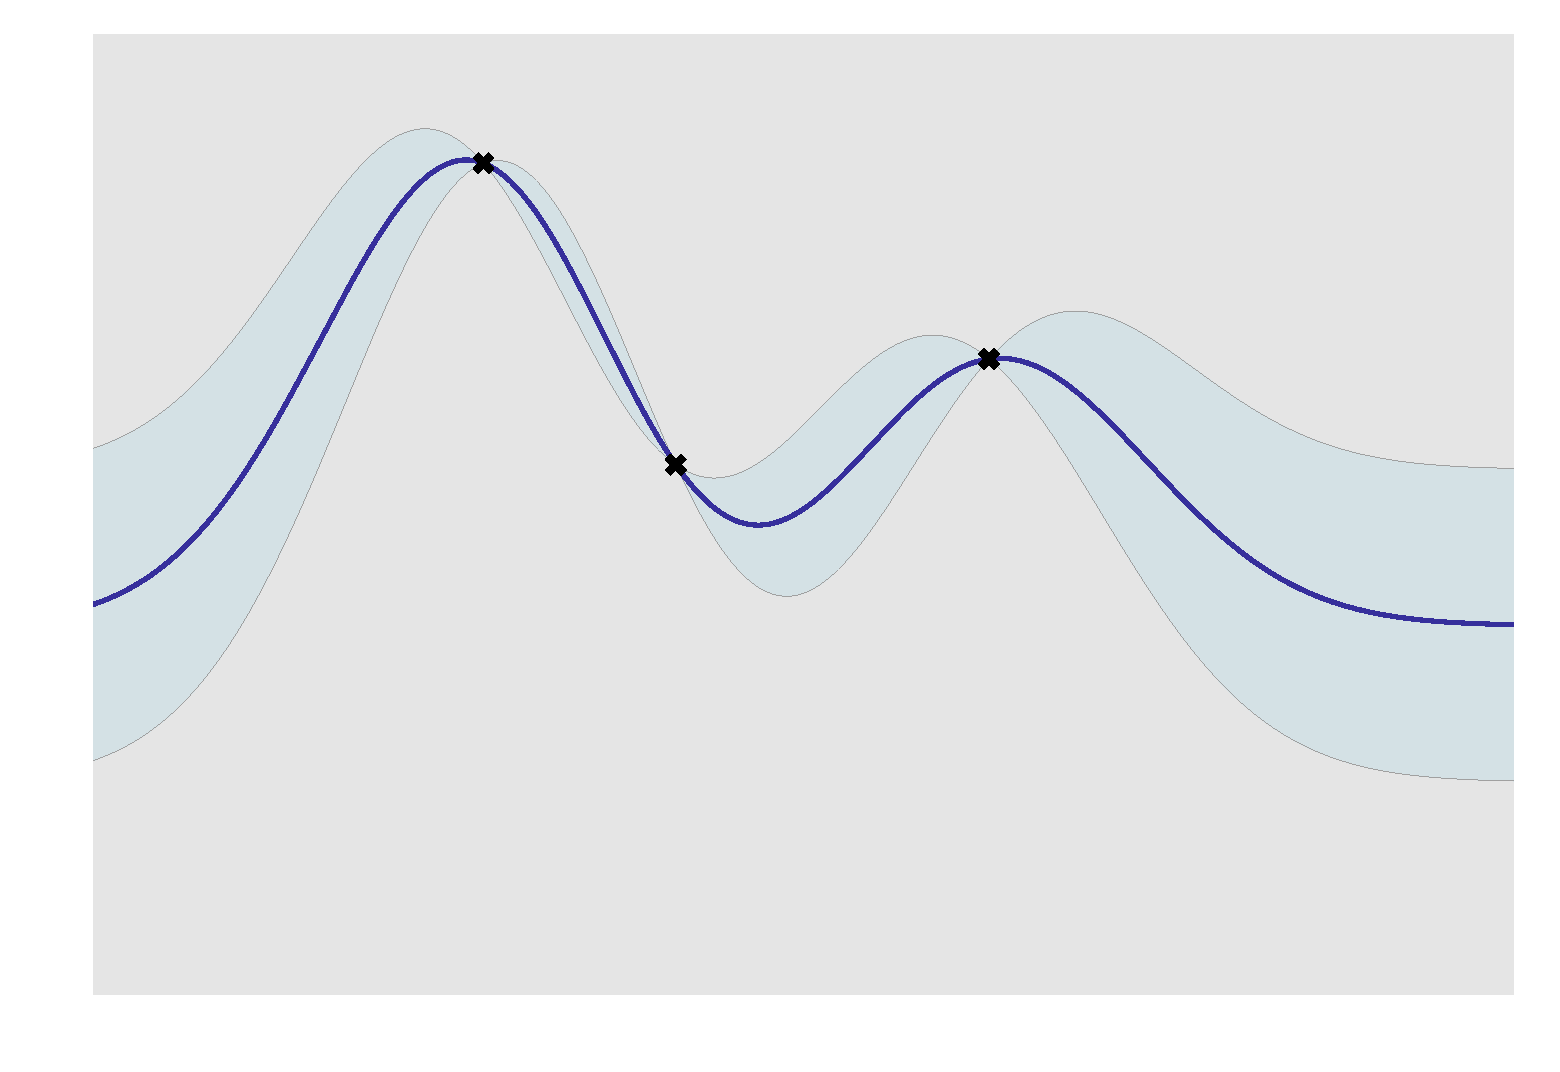
\includegraphics[width=.7\linewidth, height=0.7\textheight, keepaspectratio=true]{images/acq_func_images/ts_1.pdf}};
    \node<.> [below=0.01\belowcaptionskip of img1, align=center]{Given the GP at iteration $\bocount$};
    \node<+> (img2) {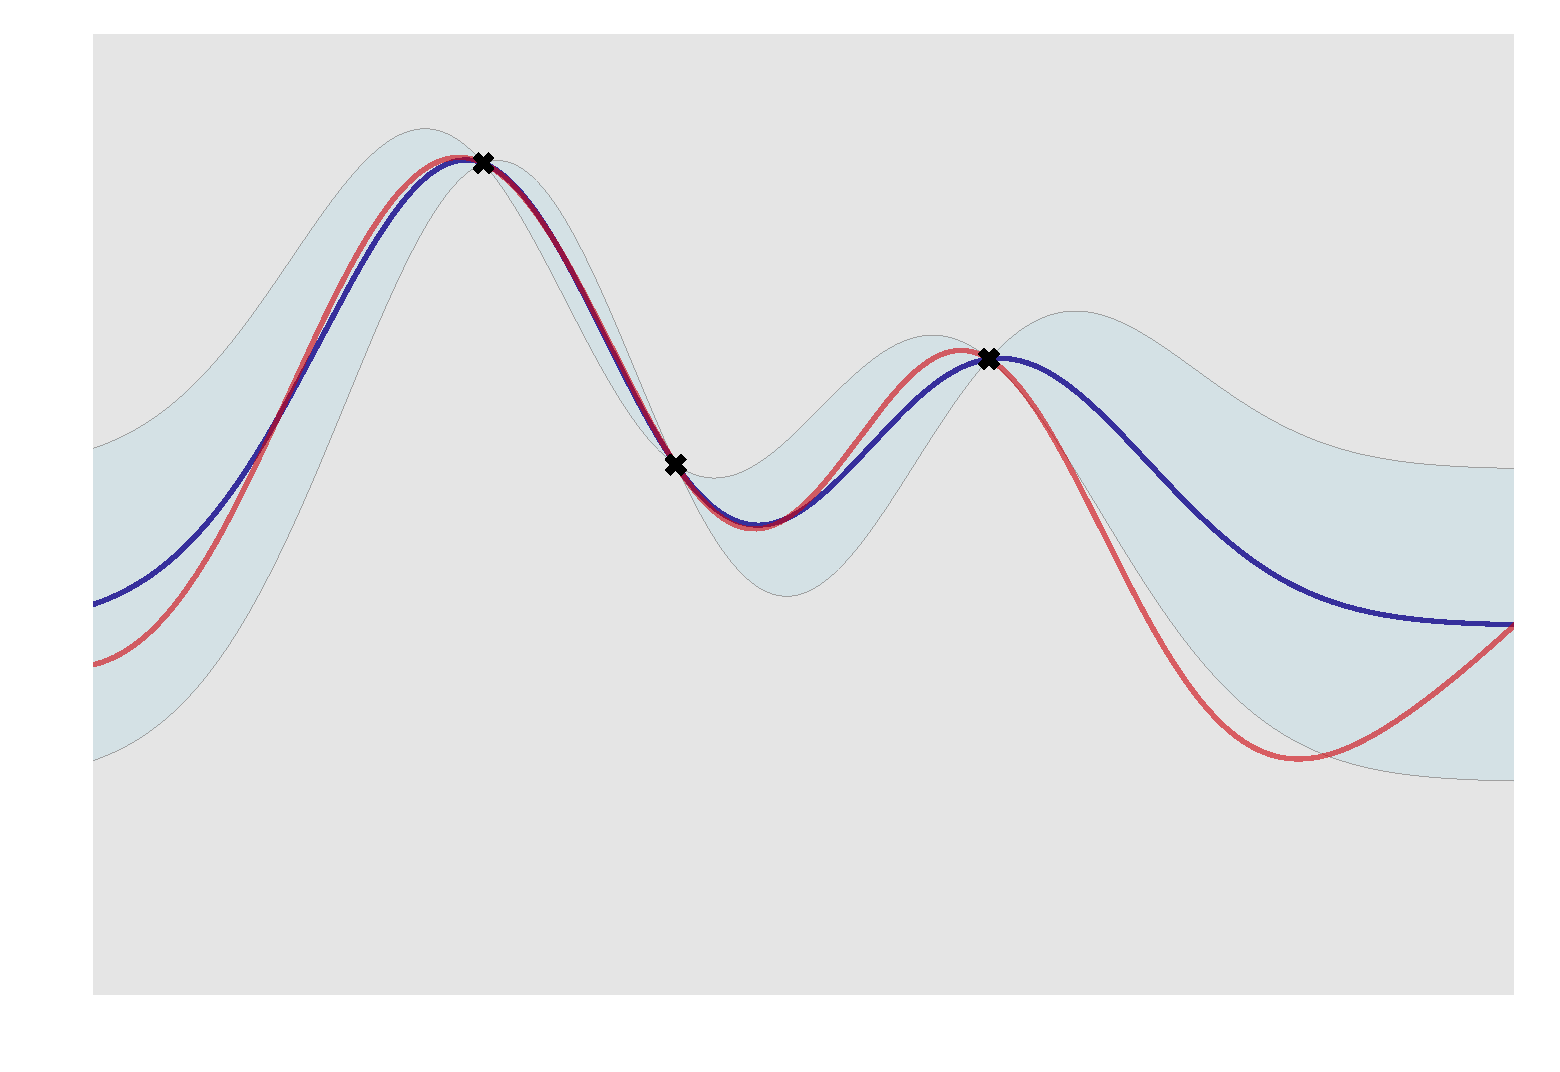
\includegraphics[width=.7\linewidth, height=0.7\textheight, keepaspectratio=true]{images/acq_func_images/ts_2.pdf}};
    \node<.> [below=0.01\belowcaptionskip of img2, align=center]{Draw a sample $g$ from the GP};
    \node<+> (img3) {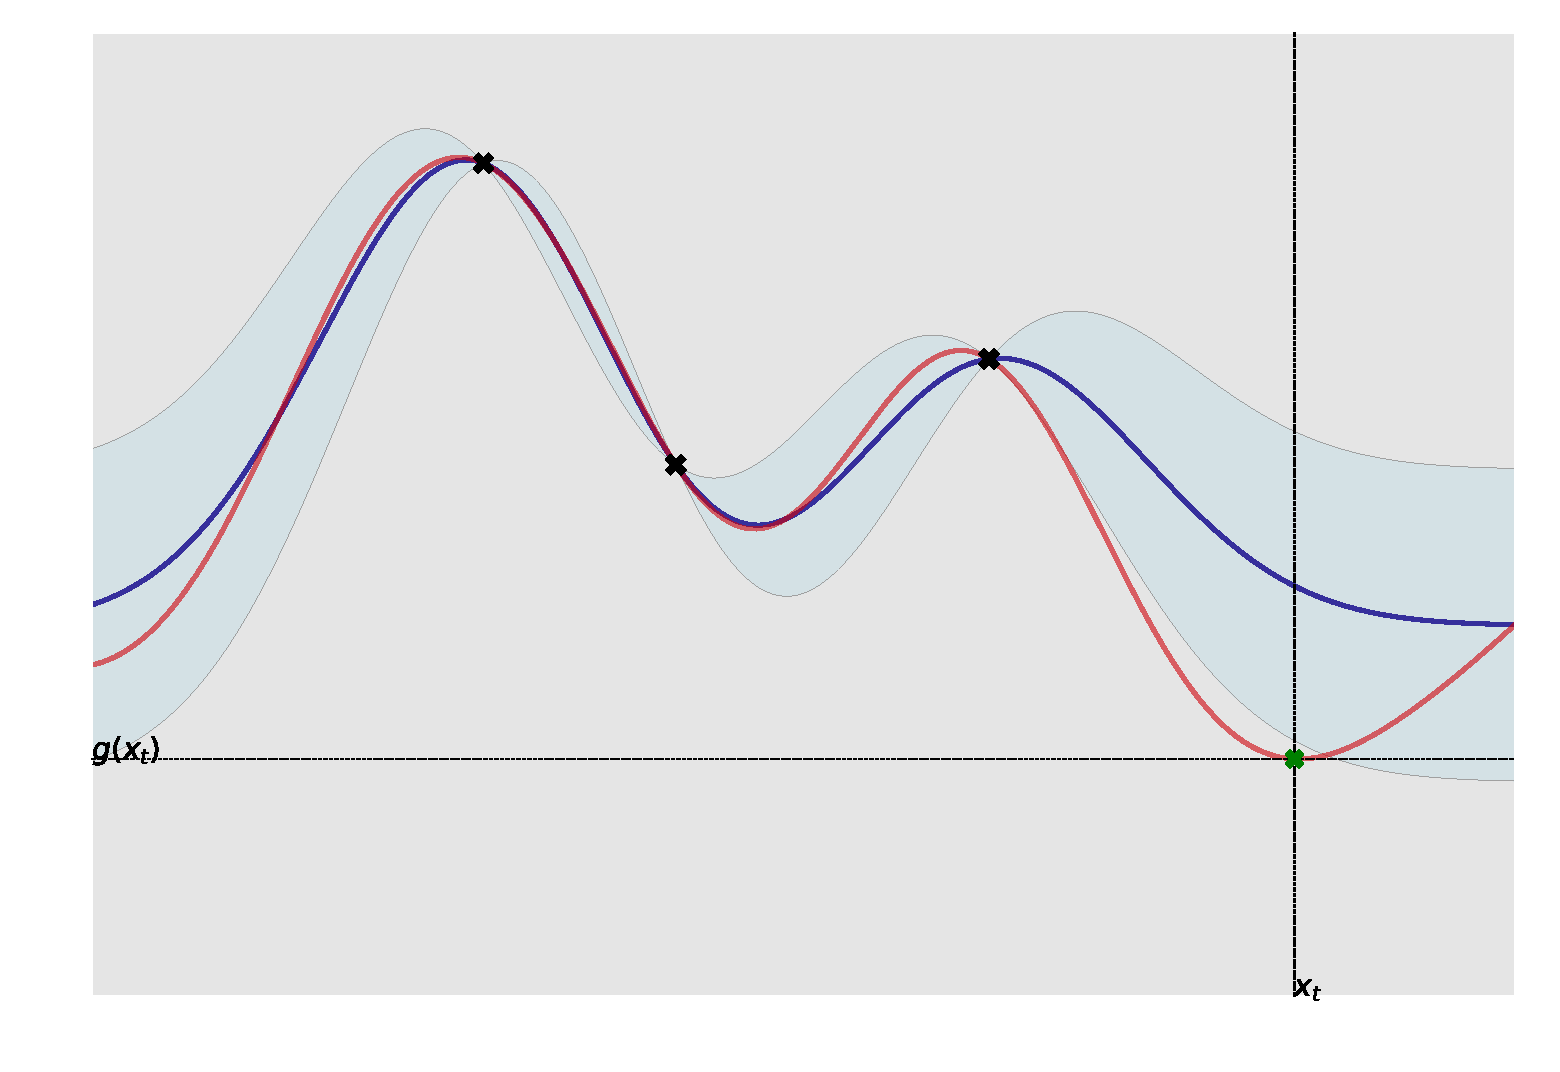
\includegraphics[width=.7\linewidth, height=0.7\textheight, keepaspectratio=true]{images/acq_func_images/ts_3.pdf}};
    \node<.> [below=0.01\belowcaptionskip of img3, align=center]{Then choose the minimum of this sample};
  \end{tikzpicture}
\end{figure}

\end{frame}
%-----------------------------------------------------------------------
\begin{frame}[c]{Basic Acquisition Functions - TS}
\framesubtitle{Thompson Sampling - Choosing a candidate}

\begin{itemize}
    \item Draw a sample $g$ from the GP $\iter{\gp}$.
    \item Choose $\bonextsample=\argmin_{\conf\in\pcs}(g(\conf))$
\end{itemize}
\end{frame}
%-----------------------------------------------------------------------
\begin{frame}[c]{Basic Acquisition Functions - TS}
\framesubtitle{Thompson Sampling - Choosing a candidate}
\begin{center}
\begin{minipage}{0.75\textwidth}
\comment{Fix algorithm numbering}
\begin{algorithm}[H]
    %\DontPrintSemicolon
    \LinesNumbered
    \SetAlgoLined
    \setcounter{AlgoLine}{0}
    \SetKwInOut{Require}{Require}
    \SetKwInOut{Result}{Result}
    
    \Require{Initial dataset $\iter[0]{\dataset}$, budget $\bobudget$}
    \Result{$\iter[\bobudget]{\dataset}$ and $\finconf$}
    
    $\iter[0]{\dataset}\leftarrow\varnothing$,$\quad\gp(\cdot \given \iter[0]{\dataset})\leftarrow\gp(0, \kernel)$\;
    
    \For{$\bocount=1$ \KwTo $\bobudget$}{
    
        Fit $\iter{\gp}=\gp(\cdot \given \iter[\bocount-1]{\dataset})$\;
    
        Sample $g\sim\iter{\gp}$\;
    
        $\bonextsample\leftarrow\argmin_{\conf\in\pcs}g(\conf)$\;
    
        $\bonextobs\leftarrow \text{ Query }\cost\text{ at }\bonextsample$\;
    
        $\iter{\dataset}\leftarrow\iter[\bocount-1]{\dataset}\cup\{\langle\bonextsample,\bonextobs\rangle\}$\;}
    \caption{Thompson Sampling on a GP}
\end{algorithm}
\end{minipage}
\end{center}
%\comment{Source: Paper, Kandasamy et al, http://proceedings.mlr.press/v84/kandasamy18a/kandasamy18a.pdf}
\end{frame}
%-----------------------------------------------------------------------
% \begin{frame}[c]{Basic Acquisition Functions - TS}
% \framesubtitle{Thompson Sampling - Features}
% \comment{Replace with table of comparisons}
% \begin{itemize}
%     \item Not an acquisition function, but an acquisition \textit{method} instead.
%     \item Well-known theoretical bounds on maximum and minimum regret.
%     \item Simple Bayesian approach to solving the multi-armed bandit problem.
% \end{itemize}
% \end{frame}